\afterpage{
\clearpage
\begin{figure}[p]
    \centering
    \begin{subfigure}[b]{0.47\textwidth}
        \centering
        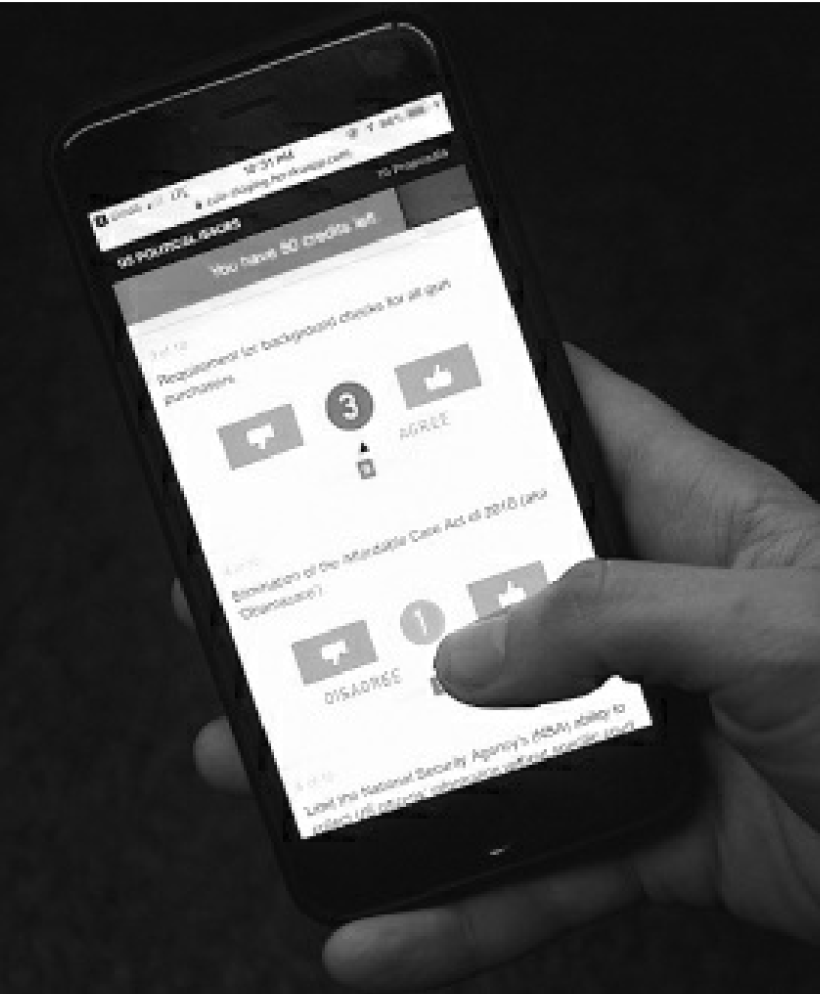
\includegraphics[width=0.67\textwidth]{content/image/curr_interface/radical_market_wedesign.png}
        \caption{Software by WeDesign, used in the first empirical QV research~\cite{quarfoot2017quadratic}. Little information is available about the software, except for an image from~\cite{posner2018radical}. In the image, each prompt has thumbs up and down icons to update the vote in the center. The remaining budget appears as a progress bar at the top.}
        \label{fig:wedesignInterface}
    \end{subfigure}
    \hspace{0.5cm}
    \begin{subfigure}[b]{0.47\textwidth}
        \centering
        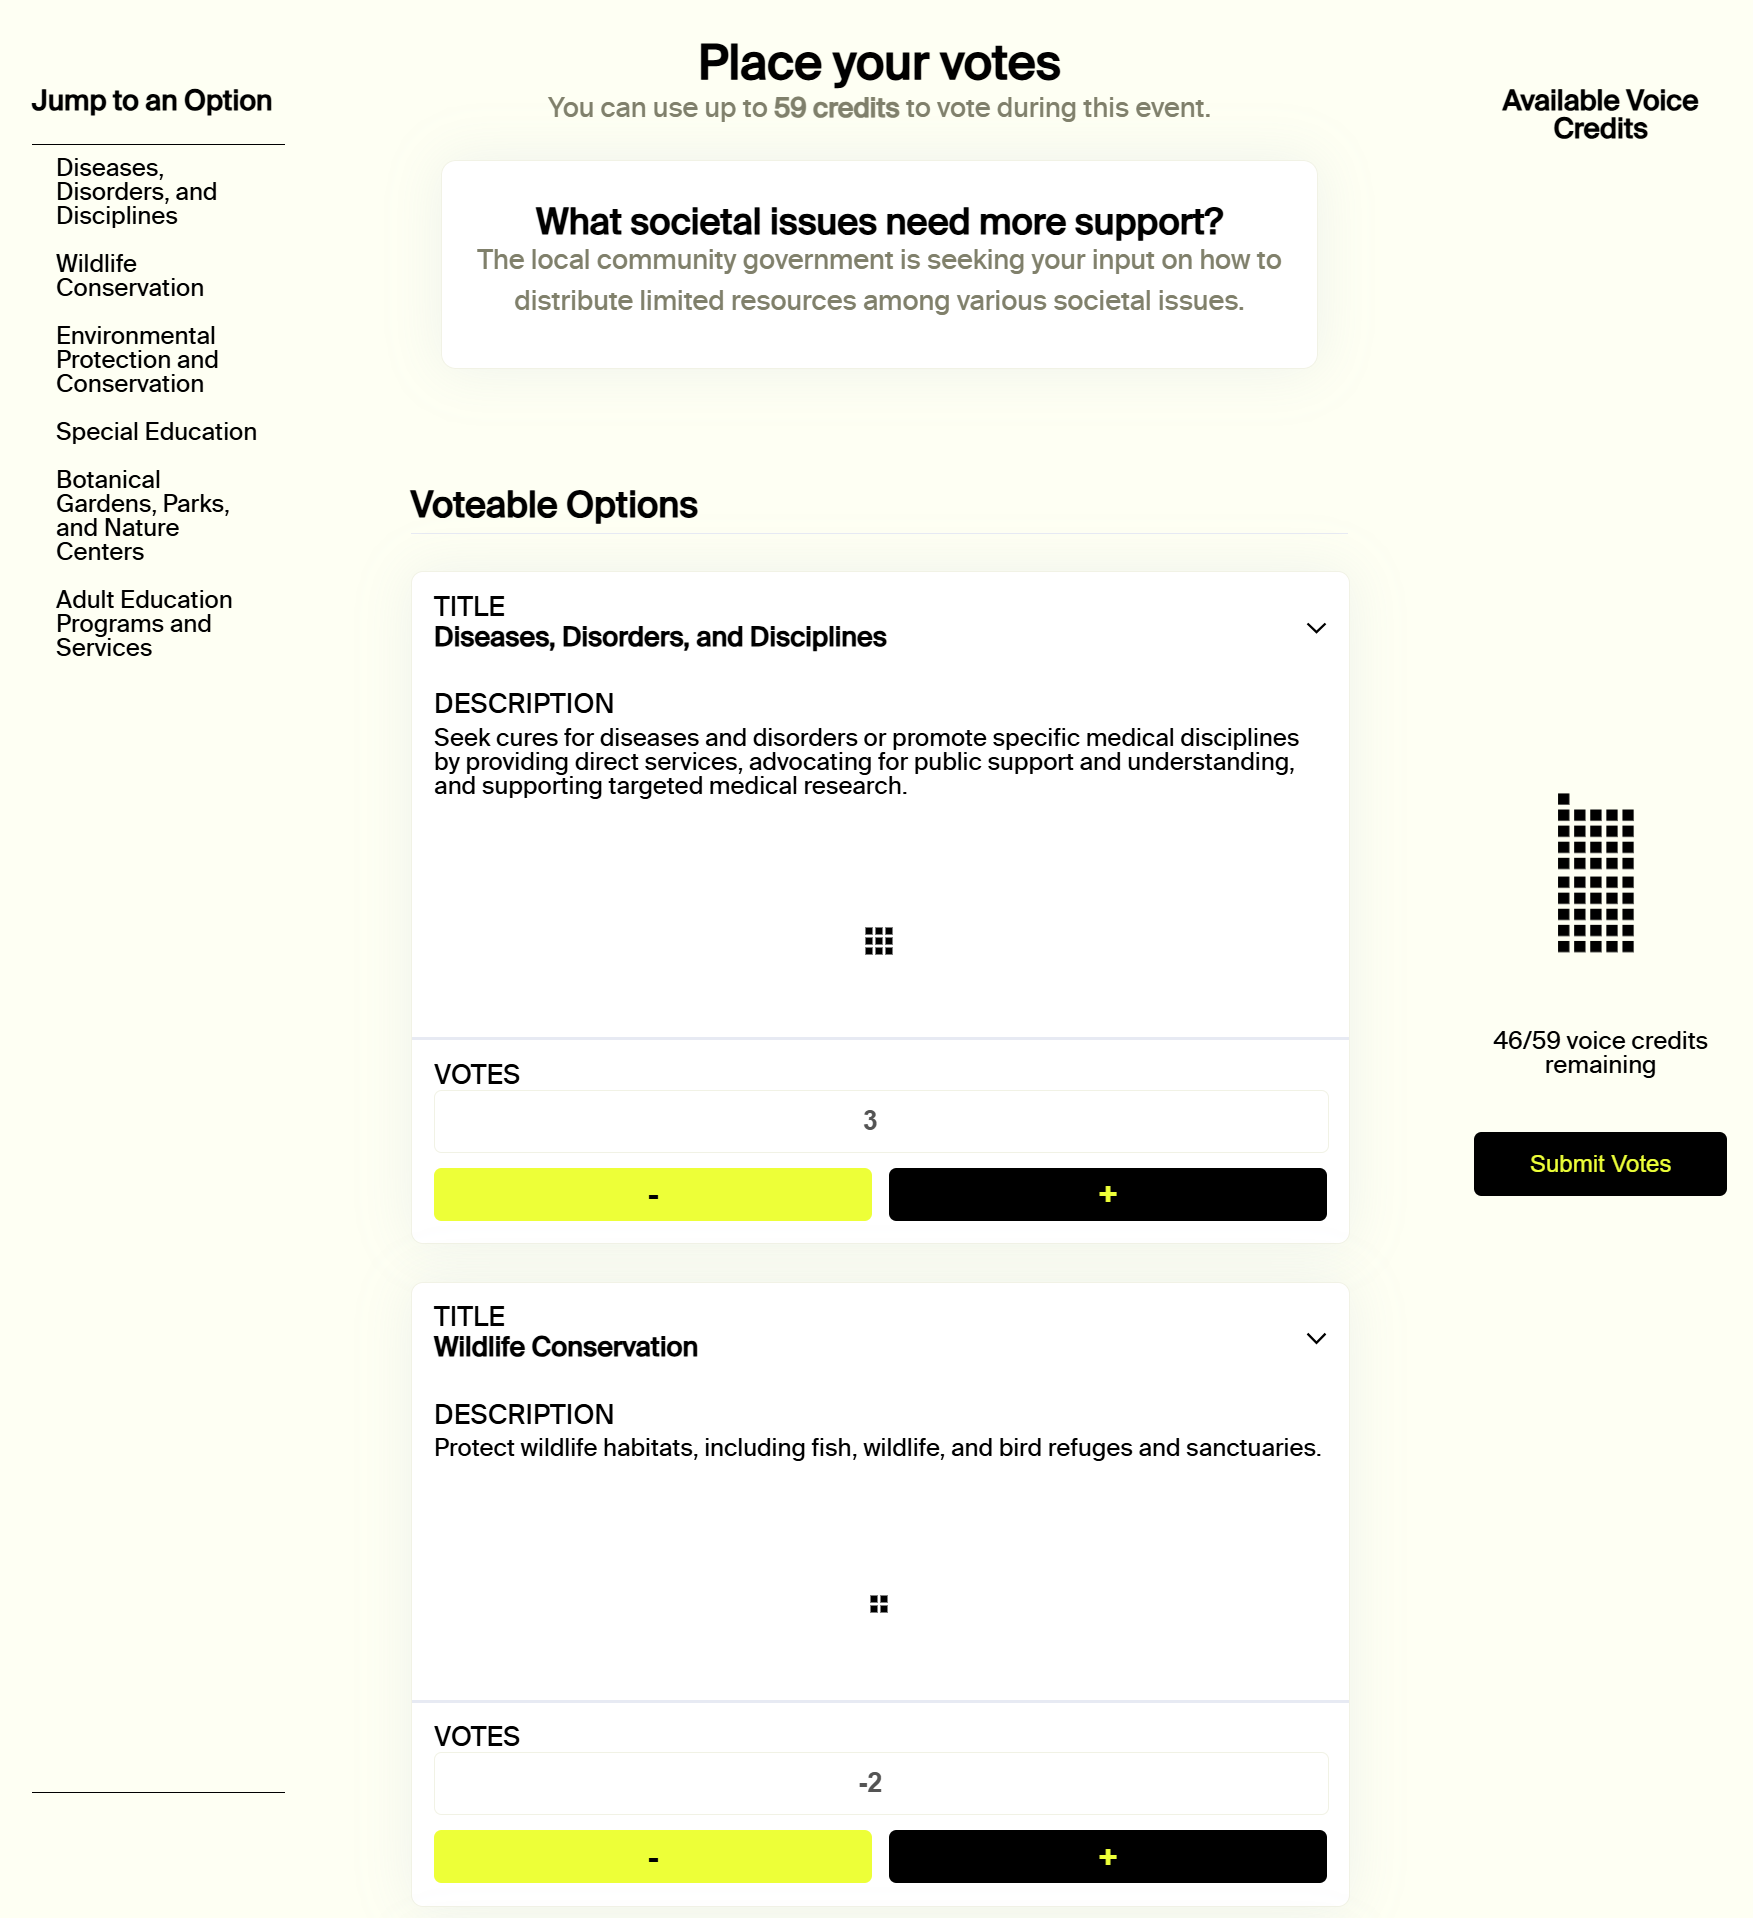
\includegraphics[width=0.72\textwidth]{content/image/curr_interface/rxc_interface.png}
        \caption{An open-sourced QV interface~\cite{RadicalxChangeQuadraticvoting2024} forked from GitCoin~\cite{ReadWhitepaperGitcoin}, used by the RadicalxChange community~\cite{RxC}. This interface presents total credits as small blocks. Votes are updated using plus and minus buttons, with numerical counts shown under each option and surface area as costs.}
        \label{fig:rxcvotingInterface}
    \end{subfigure}
    
    \vspace{0.15cm}
    
    \begin{subfigure}[b]{0.47\textwidth}
        \centering
        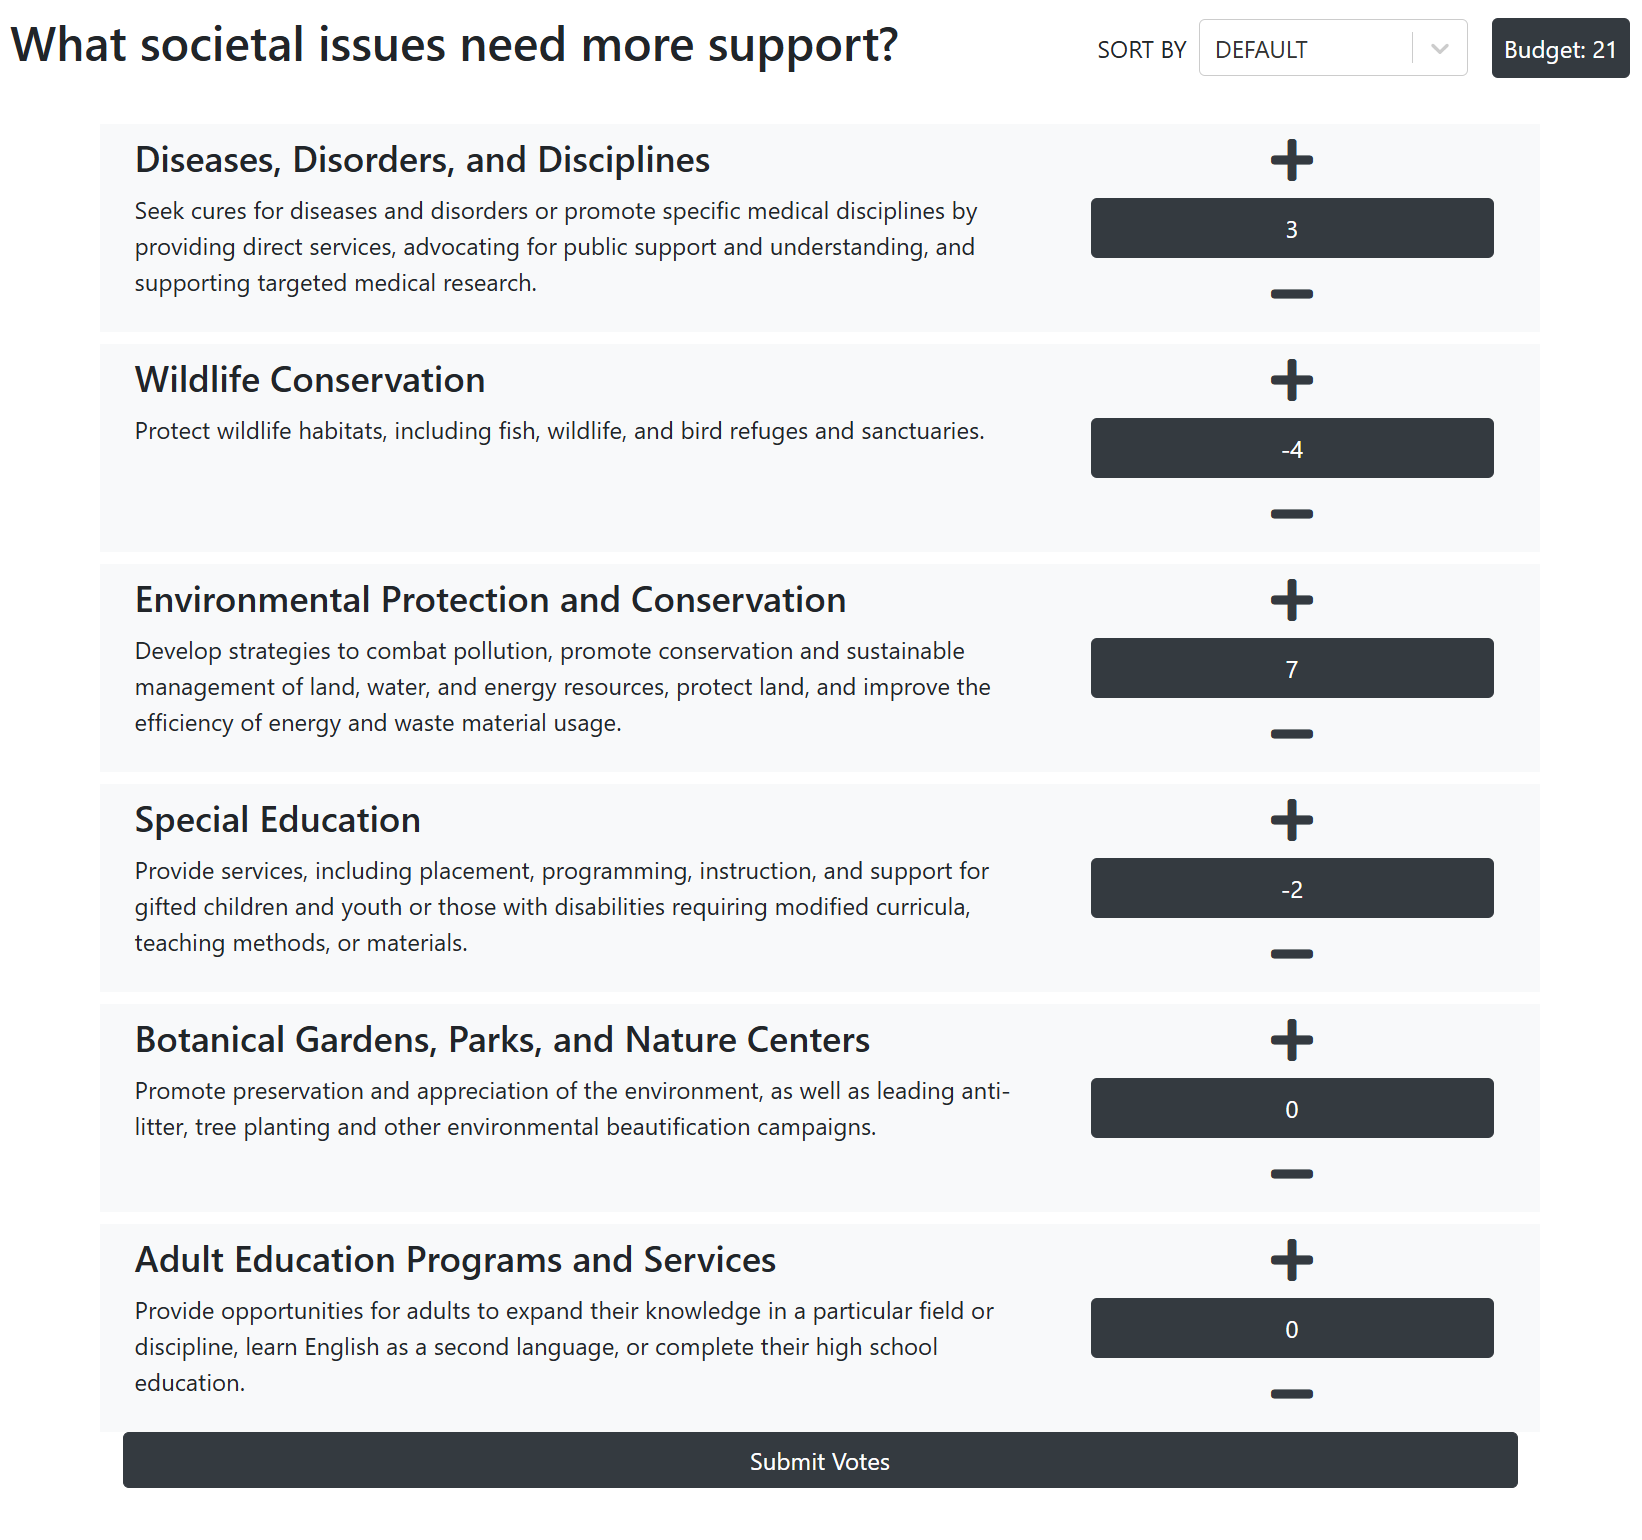
\includegraphics[width=0.72\textwidth]{content/image/curr_interface/geek.sg_interface.png}
        \caption{An open-source QV interface~\cite{yehjxraymondYehjxraymondQvapp2024} offers a publicly available service. Options show only the current number of votes, with credits displayed in the top right corner. This interface does not show the costs of votes but supports sorting options.}
        \label{fig:yehInterface}
    \end{subfigure}
    \hspace{0.5cm}
    \begin{subfigure}[b]{0.47\textwidth}
        \centering
        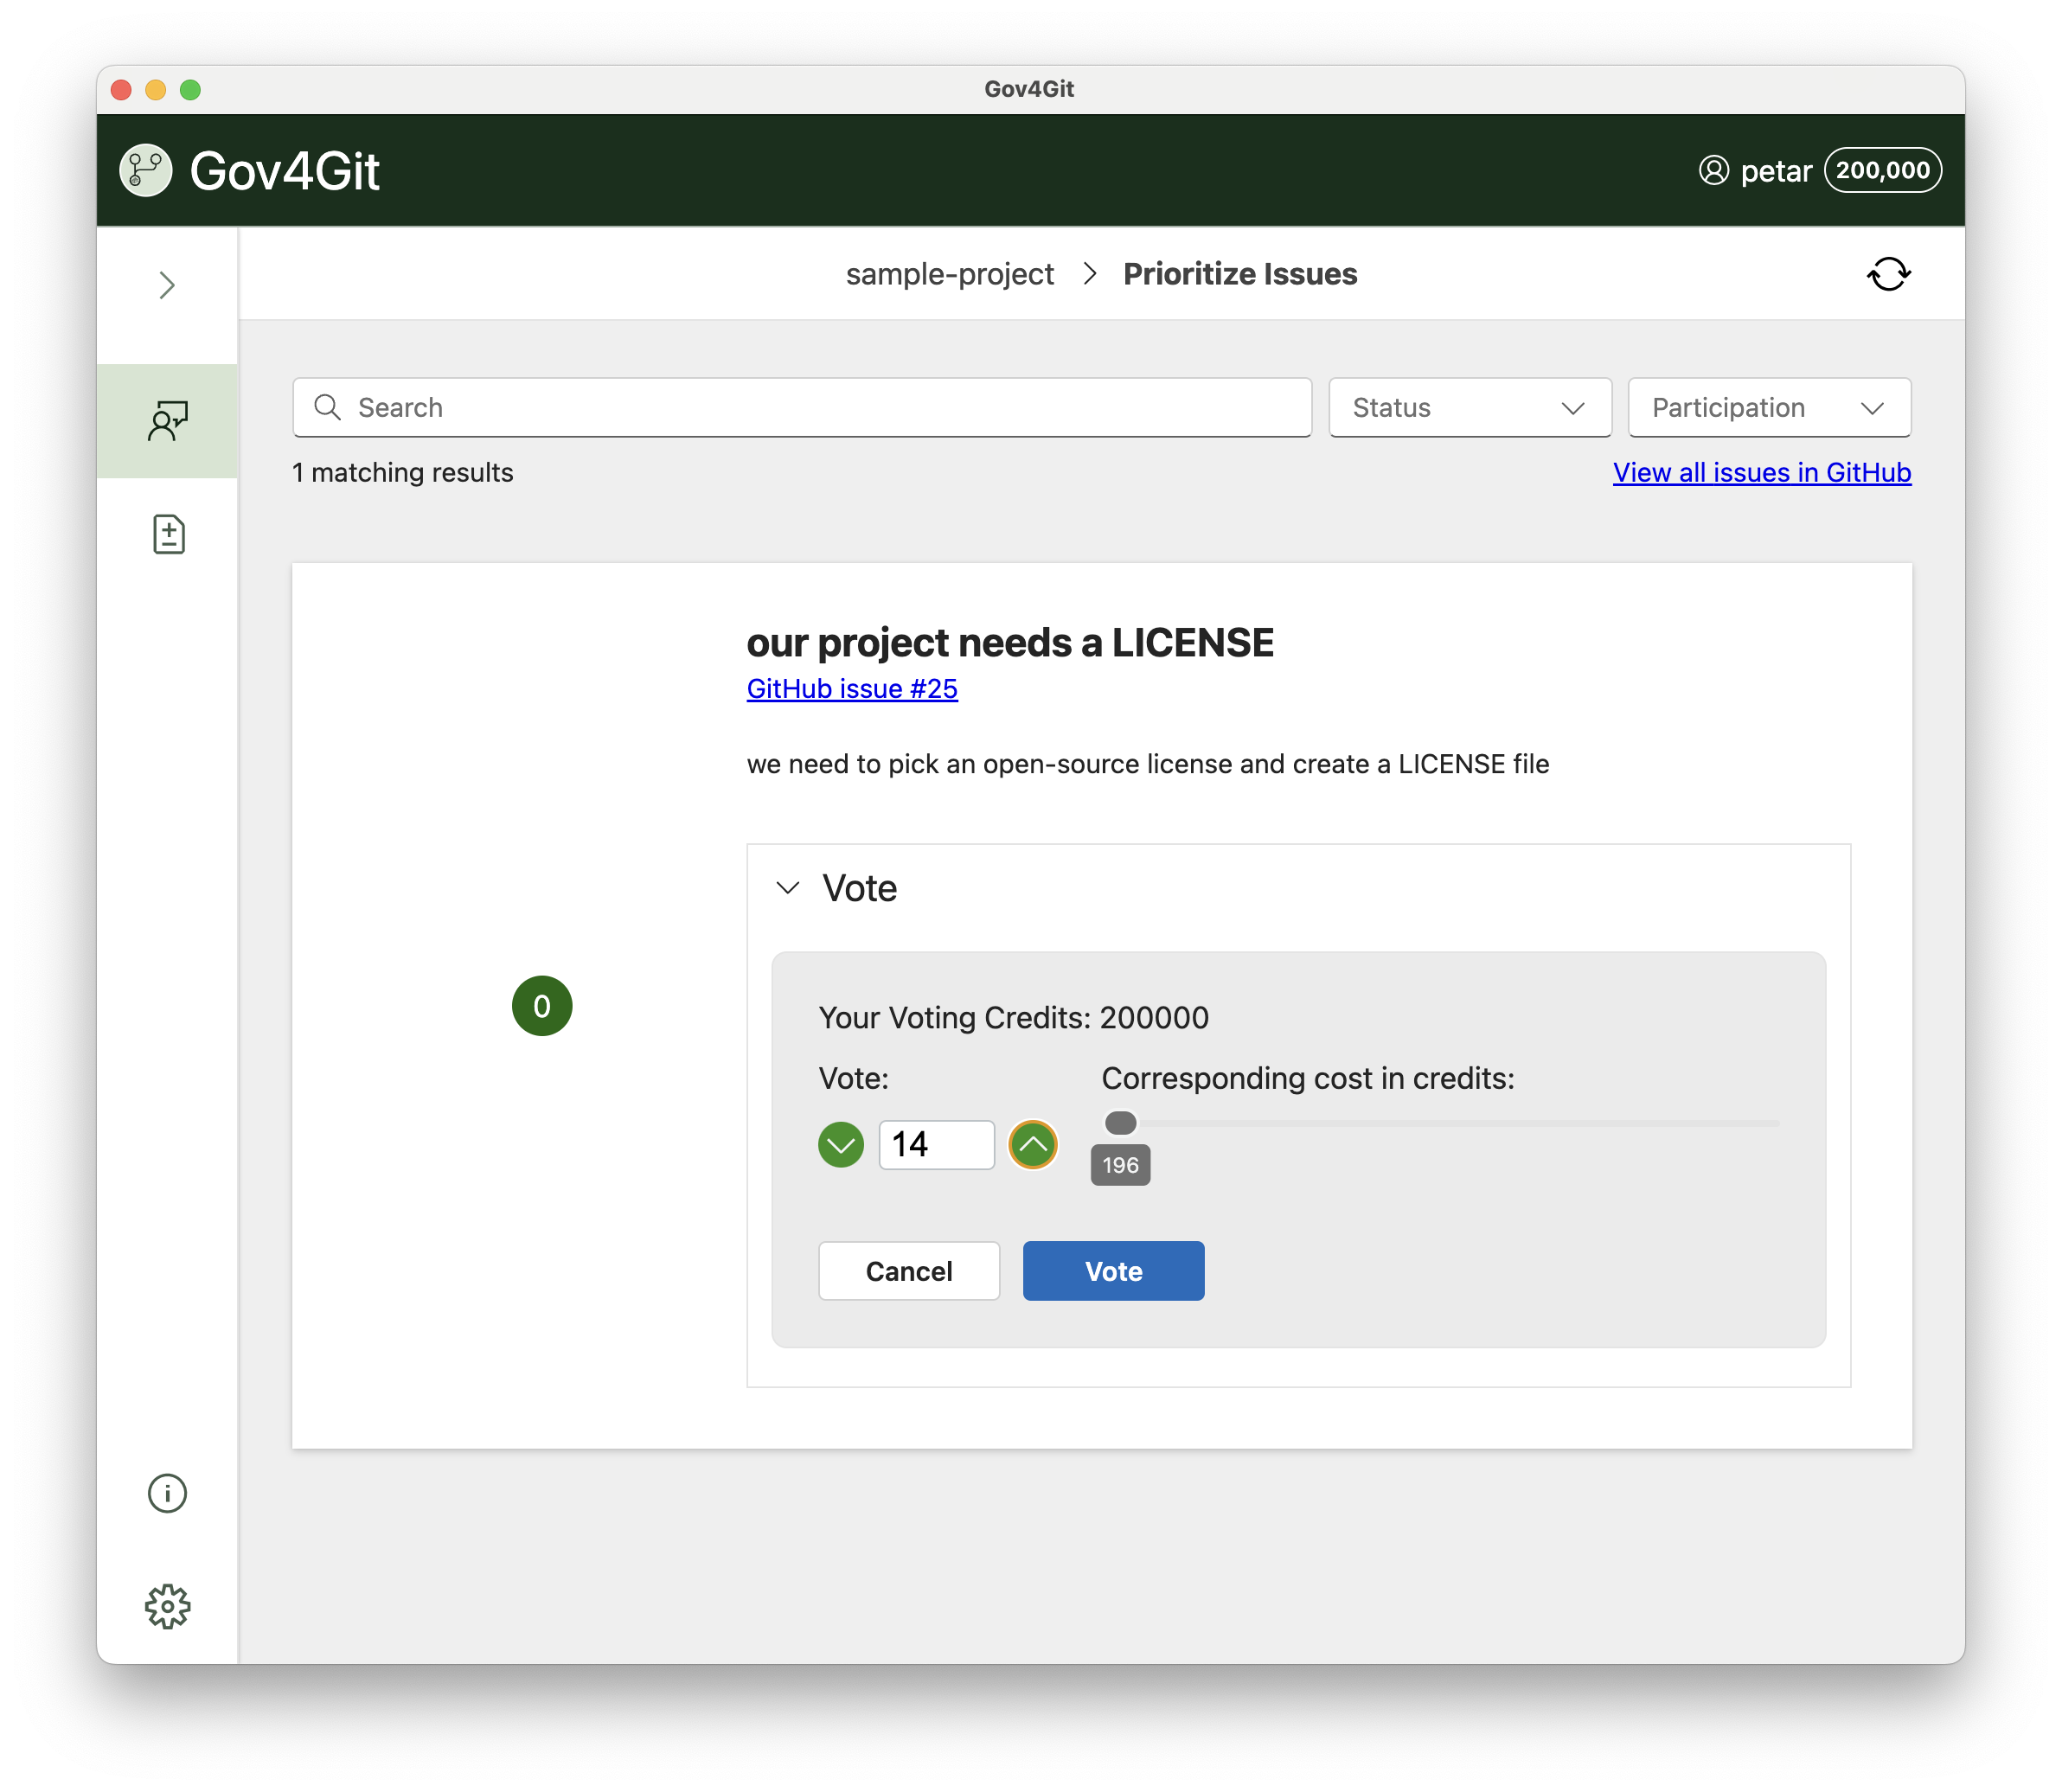
\includegraphics[width=0.72\textwidth]{content/image/curr_interface/appvote.png}
        \caption{The interface designed for gov4git~\cite{Gov4gitDecentralizedPlatform2023} updates votes using arrows under each option, with the associated cost shown as a percentage bar to the right. A search bar exists for searching specific pull requests or issues.}
        \label{fig:gov4gitInterface}
    \end{subfigure}
    
    \vspace{0.2cm}
    
    \begin{subfigure}[b]{0.7\textwidth}
        \centering
        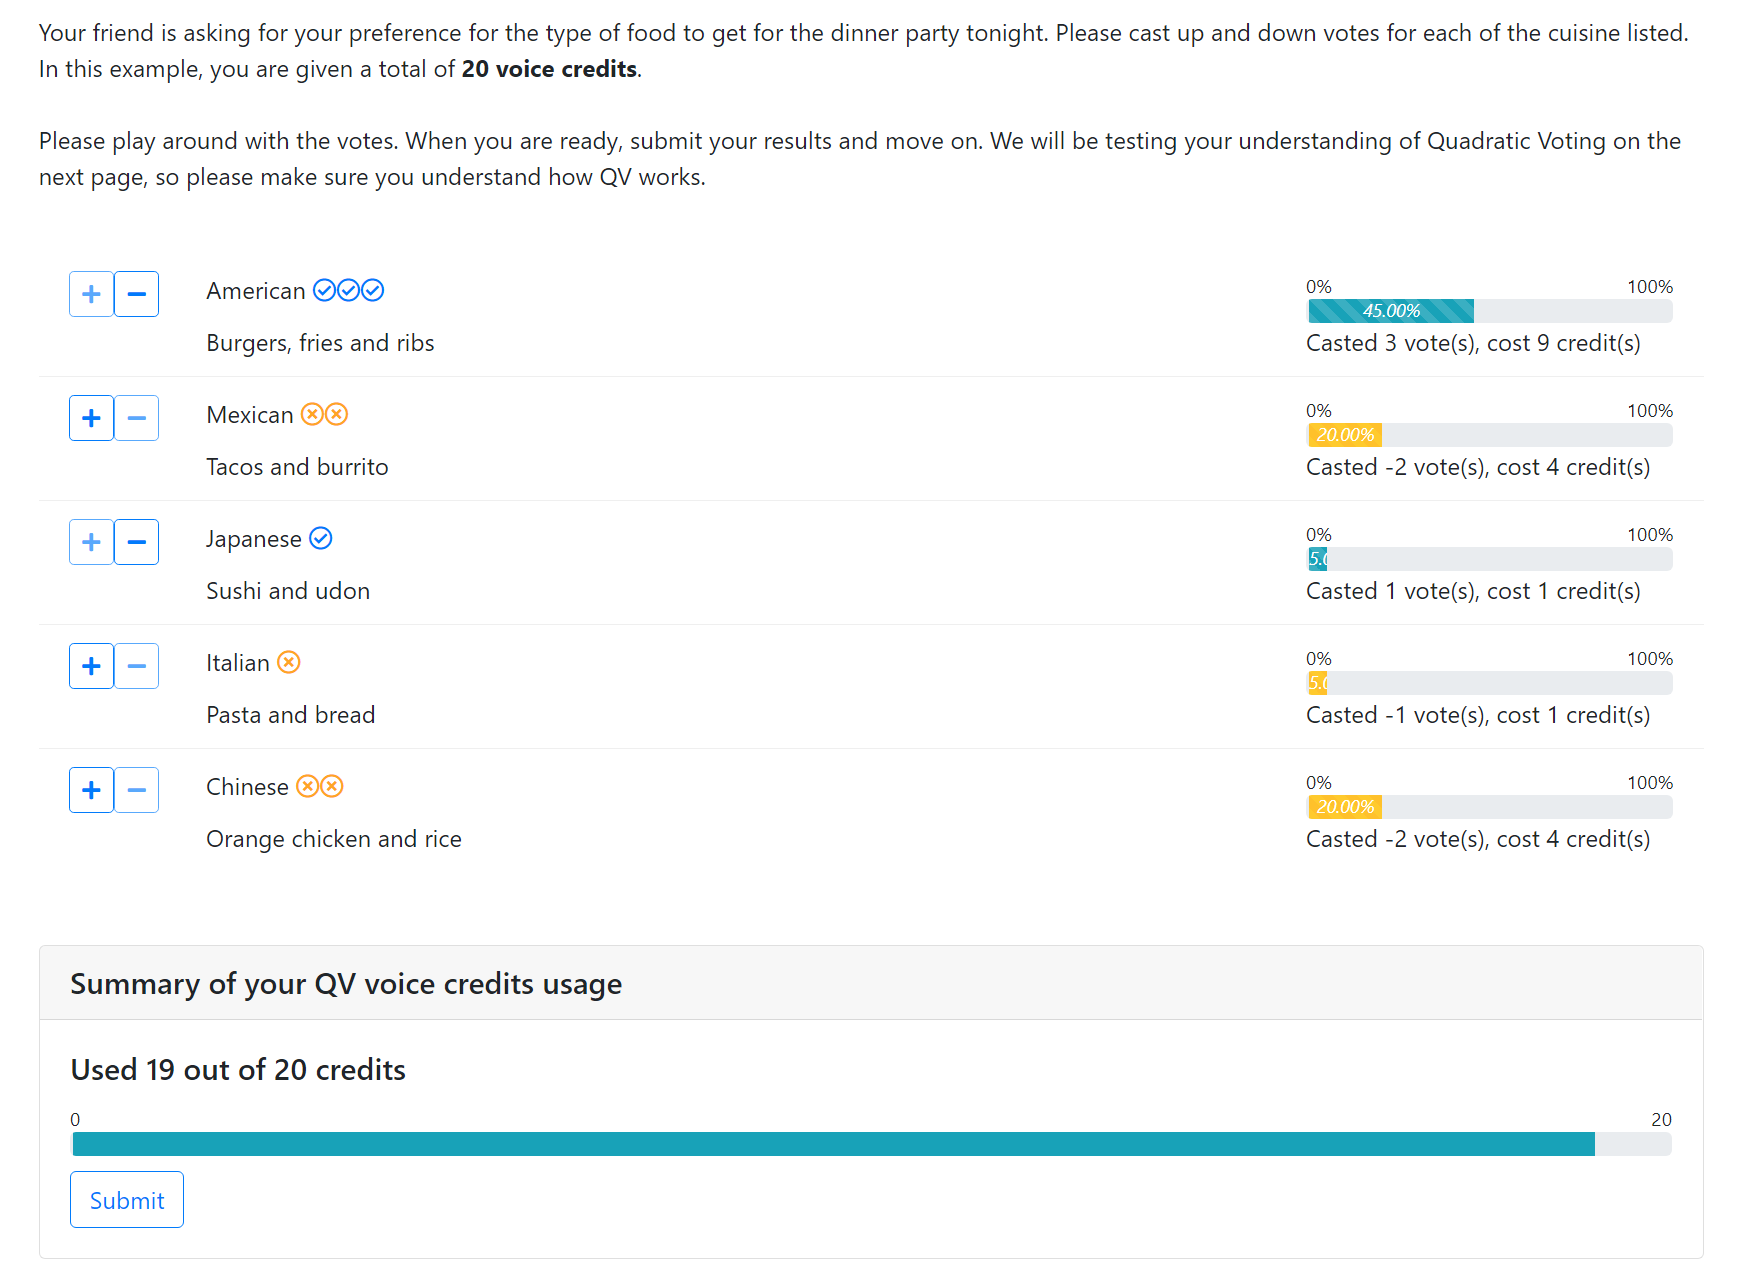
\includegraphics[width=0.50\textwidth]{content/image/curr_interface/cheng_qv.png}
        \caption{The interface used in the research by~\textcite{chengCanShowWhat2021} employs the most visual components. Icons depict the current number of votes, with progress bars signifying the current spending.}
        \label{fig:chengInterface}
    \end{subfigure}
    
    \caption{Recent interface implementations for applications using quadratic mechanism.}
    \label{fig:qv_interface_external}
\end{figure}
\clearpage
}

\section{Interface Design}
\label{sec:interfaceDesign}
Since there are no prior studies and standard interfaces for tools using the quadratic mechanism, we designed, iterated, and developed an two-phase interface for QS based on the prior literature and multiple iterations. In this section, we first describe the iterative prototyping process, detail the final design of the two-phase interface, and finally, present the text-based interface designed for comparison in this study.

\subsection{QV applications interfaces in the wild and early paper prototypes}
Since QS builds upon the QV mechanism, we being our design iteration based on existing QV applications in the wild. For coherence and brevity, we chose not to describe the paper prototype iteration in depth given it's exploratory nature. 
%  and provide it in the Appendix with other alternative design considerations in Appendix~\ref{sec:appendix_interface_alternative}

Existing interfaces consist standardized components shown in Figure~\ref{fig:qv_interface_external}~\footnote{Figure~\ref{fig:gov4gitInterface} did not exist until the writing of this paper.}. All interfaces shared these key components:
\begin{itemize}
    \item Option list: A list of options contesting for votes.
    \item Vote controls: Buttons to increase and decrease votes associated with each option.
    \item Individual vote tally: A representation of votes associated with an option.
    \item Summary: An auto-generated summary of costs and remaining budget.
\end{itemize}

Most components were focused on presenting information and obtaining votes, only the summary addressed budget constraints. During our initial paper prototyping iterations (Figure~\ref{fig:qv_paper}), we tested different presentations of these components with added features to assist information organization. Pretest respondents felt QS was challenging due to identifying relative preferences among options and deciding the degree of trade-offs between options. In this study, we focus on the first challenge to inform our interface design iterations.

\begin{figure}[H]
    \centering
    \begin{subfigure}[b]{0.54\textwidth}
        \centering
        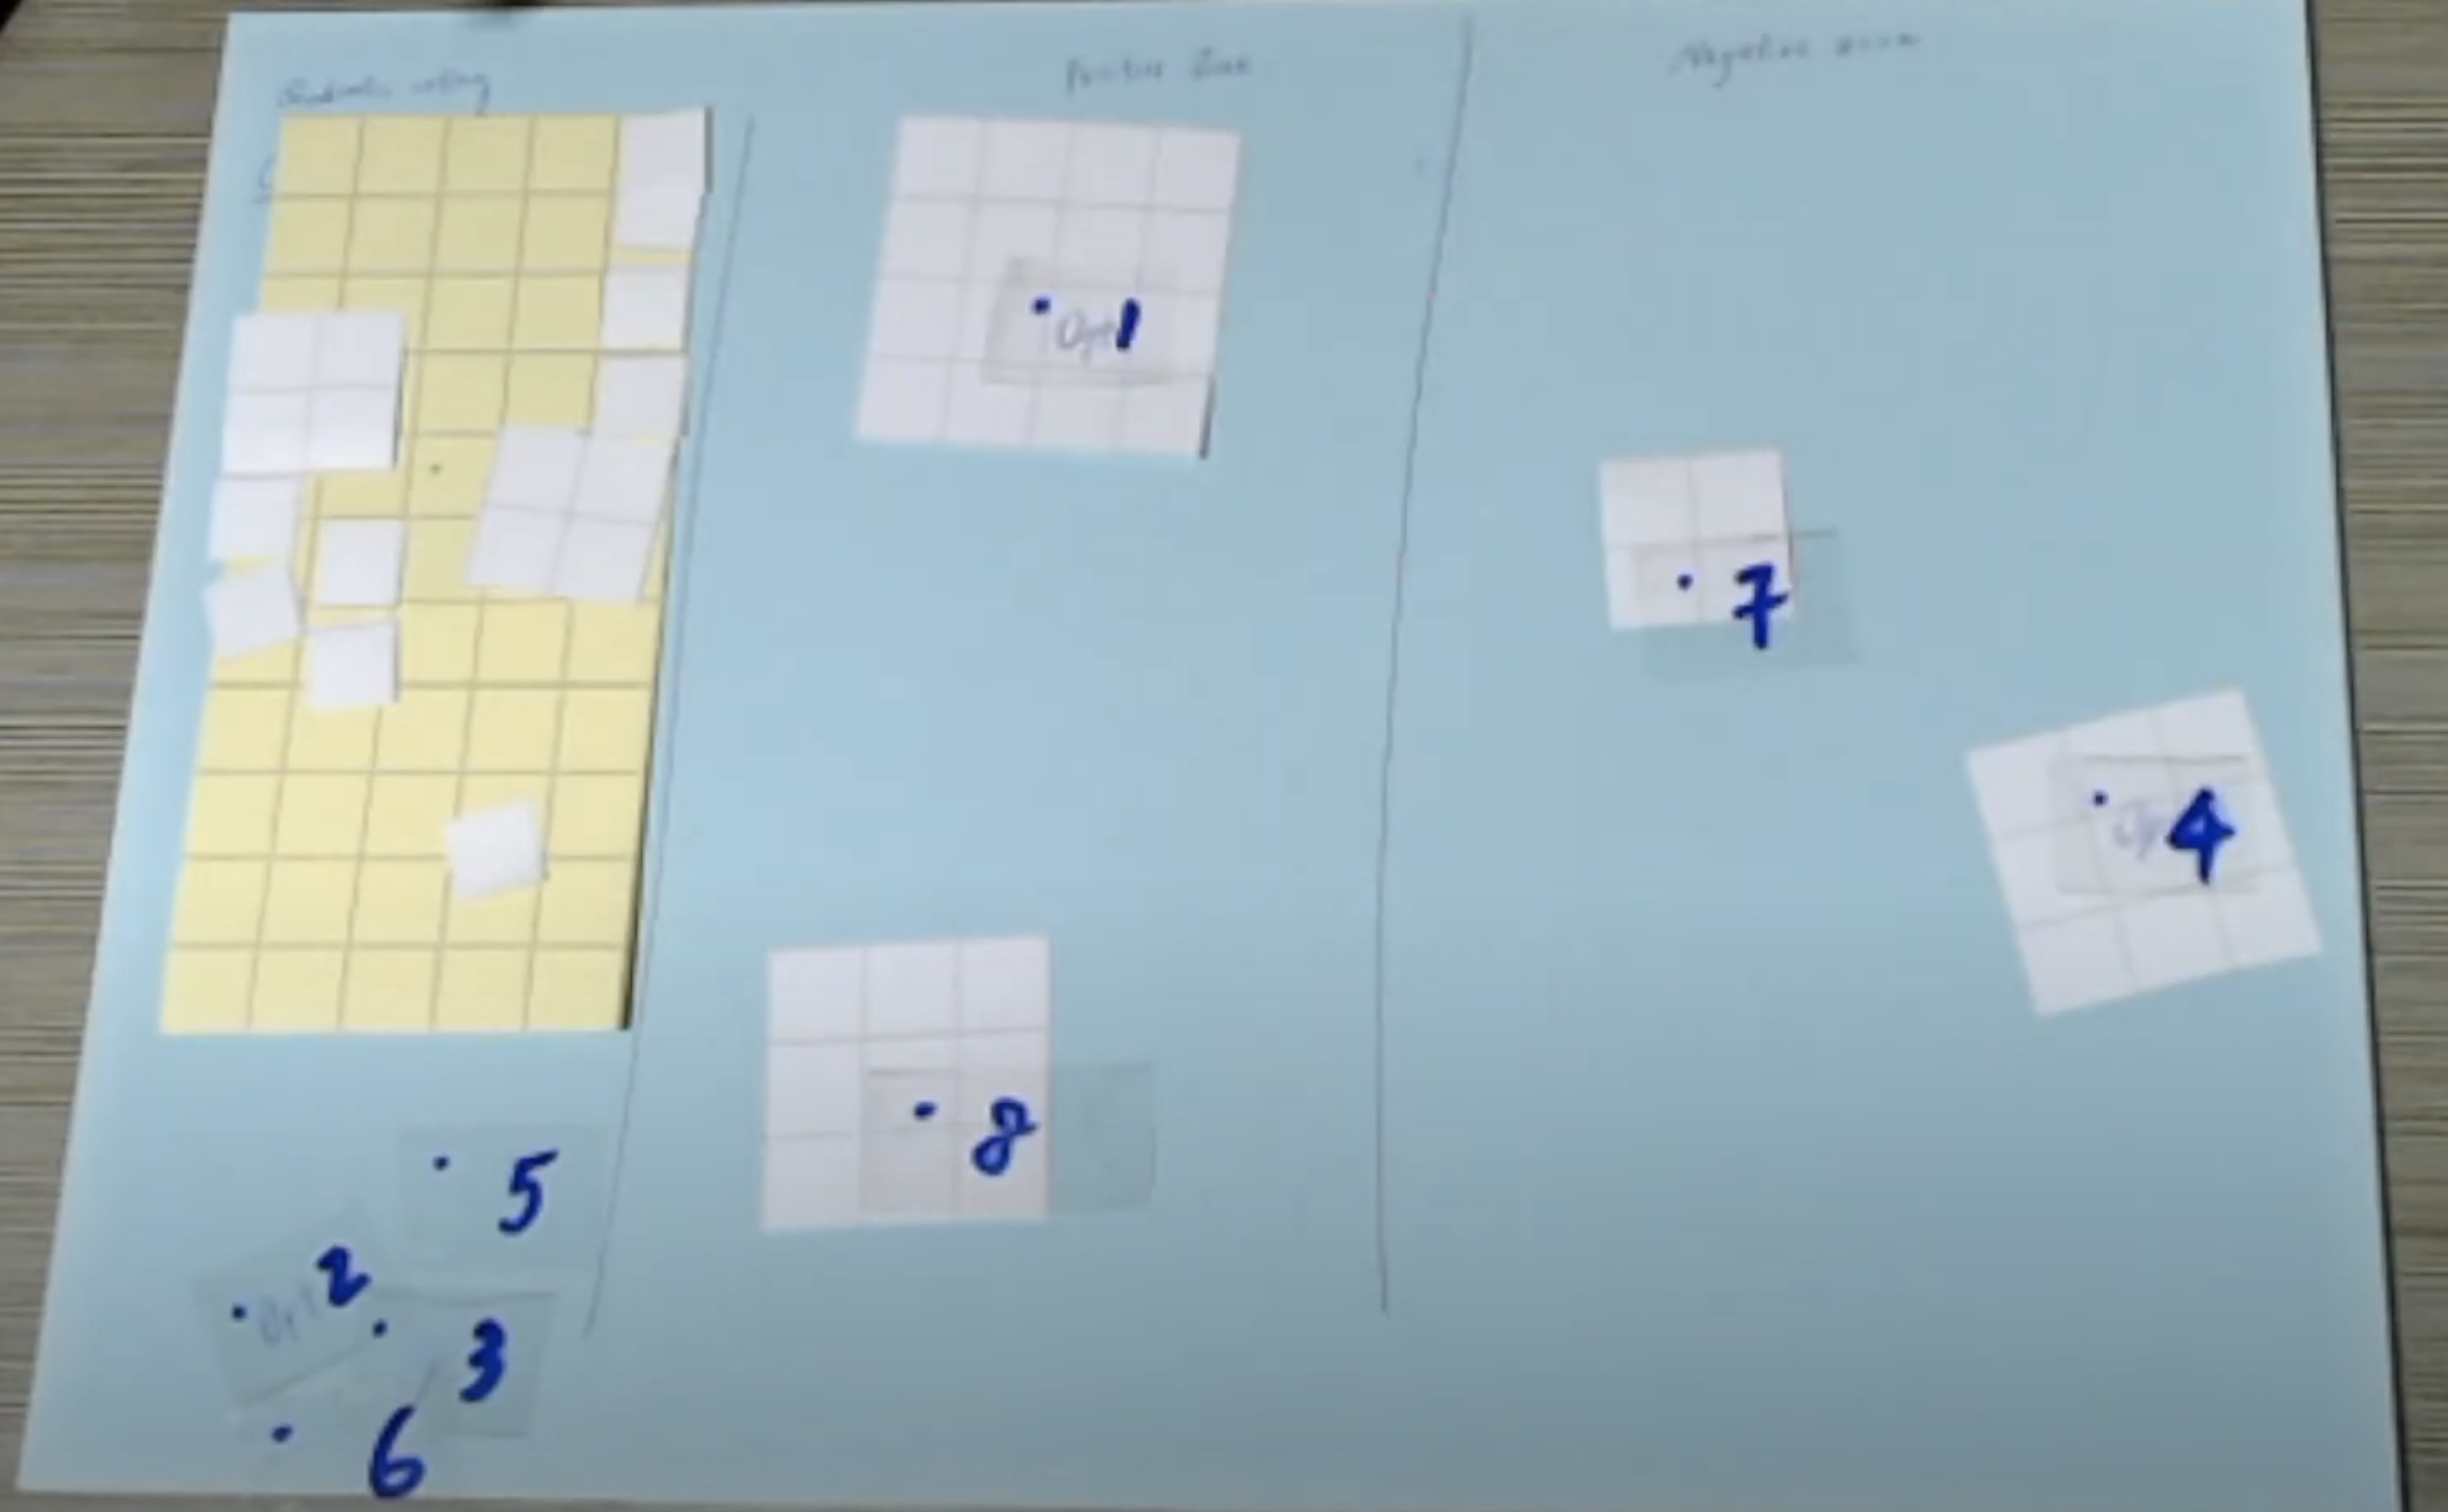
\includegraphics[width=\textwidth]{content/image/prototypes/1.2_paper_qv_single.png}
        \caption{In this paper prototype, issues are denoted by different numbers that appear on mouseover. Pretest respondents can move options anywhere in the two sections of the interface, one denoting positive and one negative. The blocks represent the cost for each option, with no indication of the number of current votes. The credits are shown in the yellow box on the left.}
        \label{fig:horizontal_paper}
    \end{subfigure}
    \hfill
    \begin{subfigure}[b]{0.42\textwidth}
        \centering
        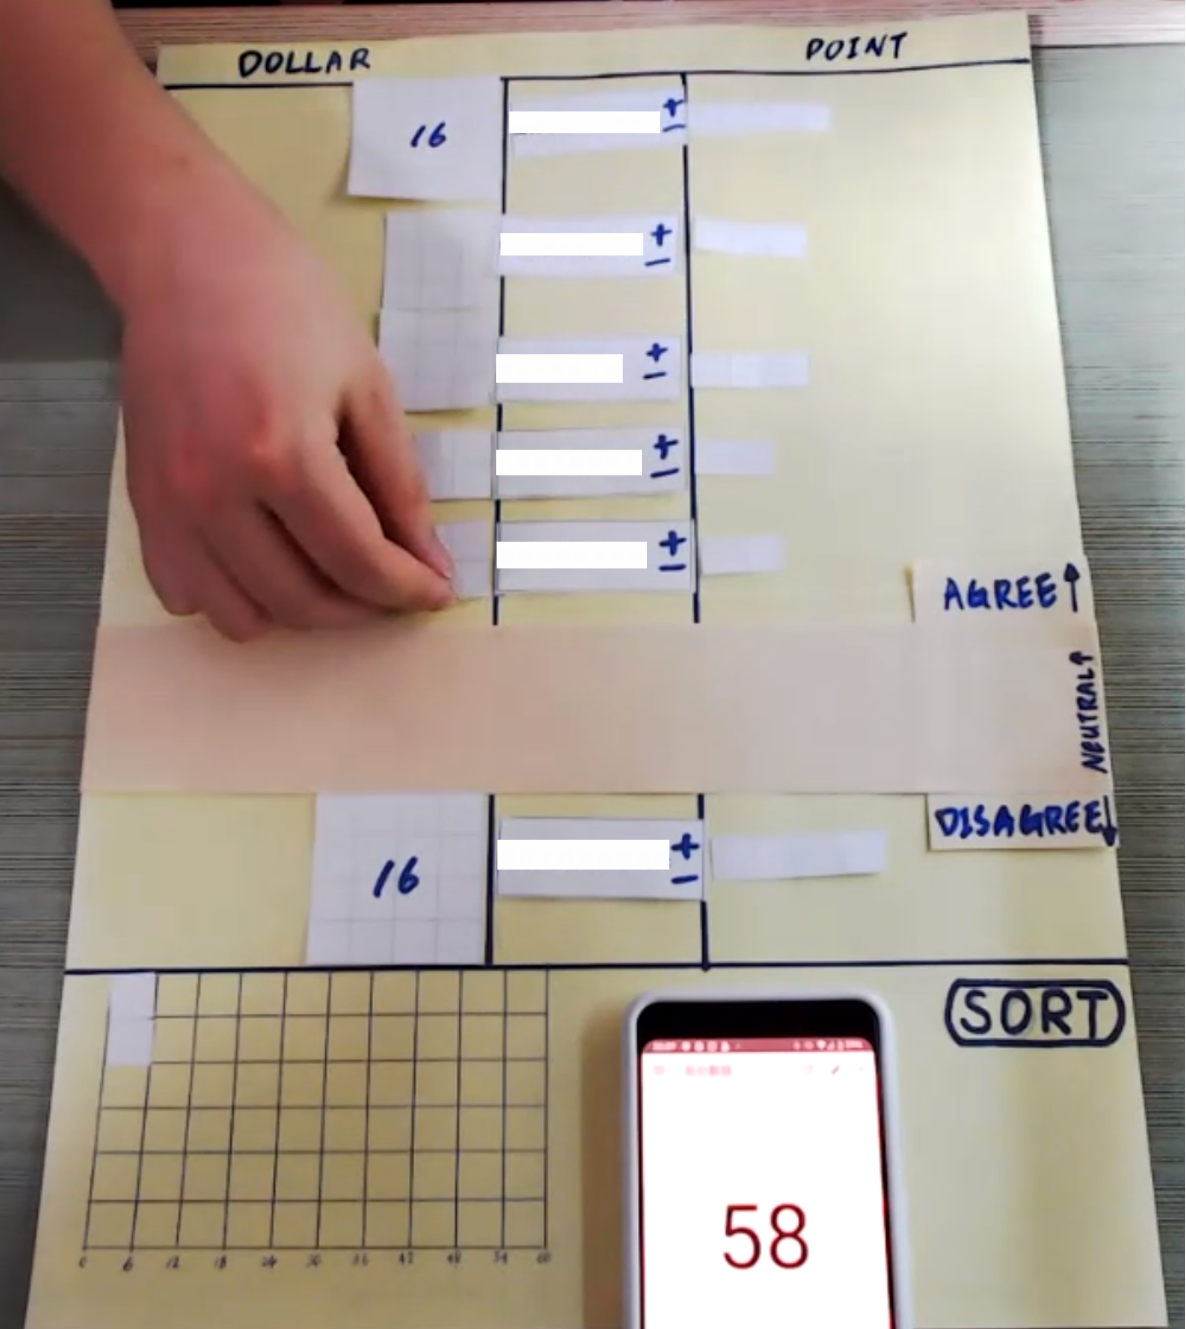
\includegraphics[width=\textwidth]{content/image/prototypes/1_paper_qv_single.png}
        \caption{This paper prototype separates the positive and negative areas with a 'band' at the center. Undecided options are placed inside this band. The cost and the votes on both sides of the interface are denoted by small blocks. The budget is shown in the yellow box below the interface with a numerical counter.}
        \label{fig:vertical_paper}
    \end{subfigure}
    \caption{Initial paper prototypes designed for QS interface}
    \label{fig:qv_paper}
\end{figure}

\subsubsection{Prototype 1: Ranking-Vote}
Considering that relative preference is often through ranking items, we tested whether ranking options before voting would help establish individual's relative preference in our prototype 1. This prototype allowed respondents to reposition options before voting. Pretests revealed that respondents rarely moved the options and questioned the necessity of full ranking, as it did not influence their QS submission. Additionally, many were unaware that options were draggable until shown. This insight indicates that full ranking is unnecessary for establishing relative preferences. Therefore, we decided to ask respondents select a subset of options instead of requiring a full rank among all options.

\begin{figure}[h]
    \centering
    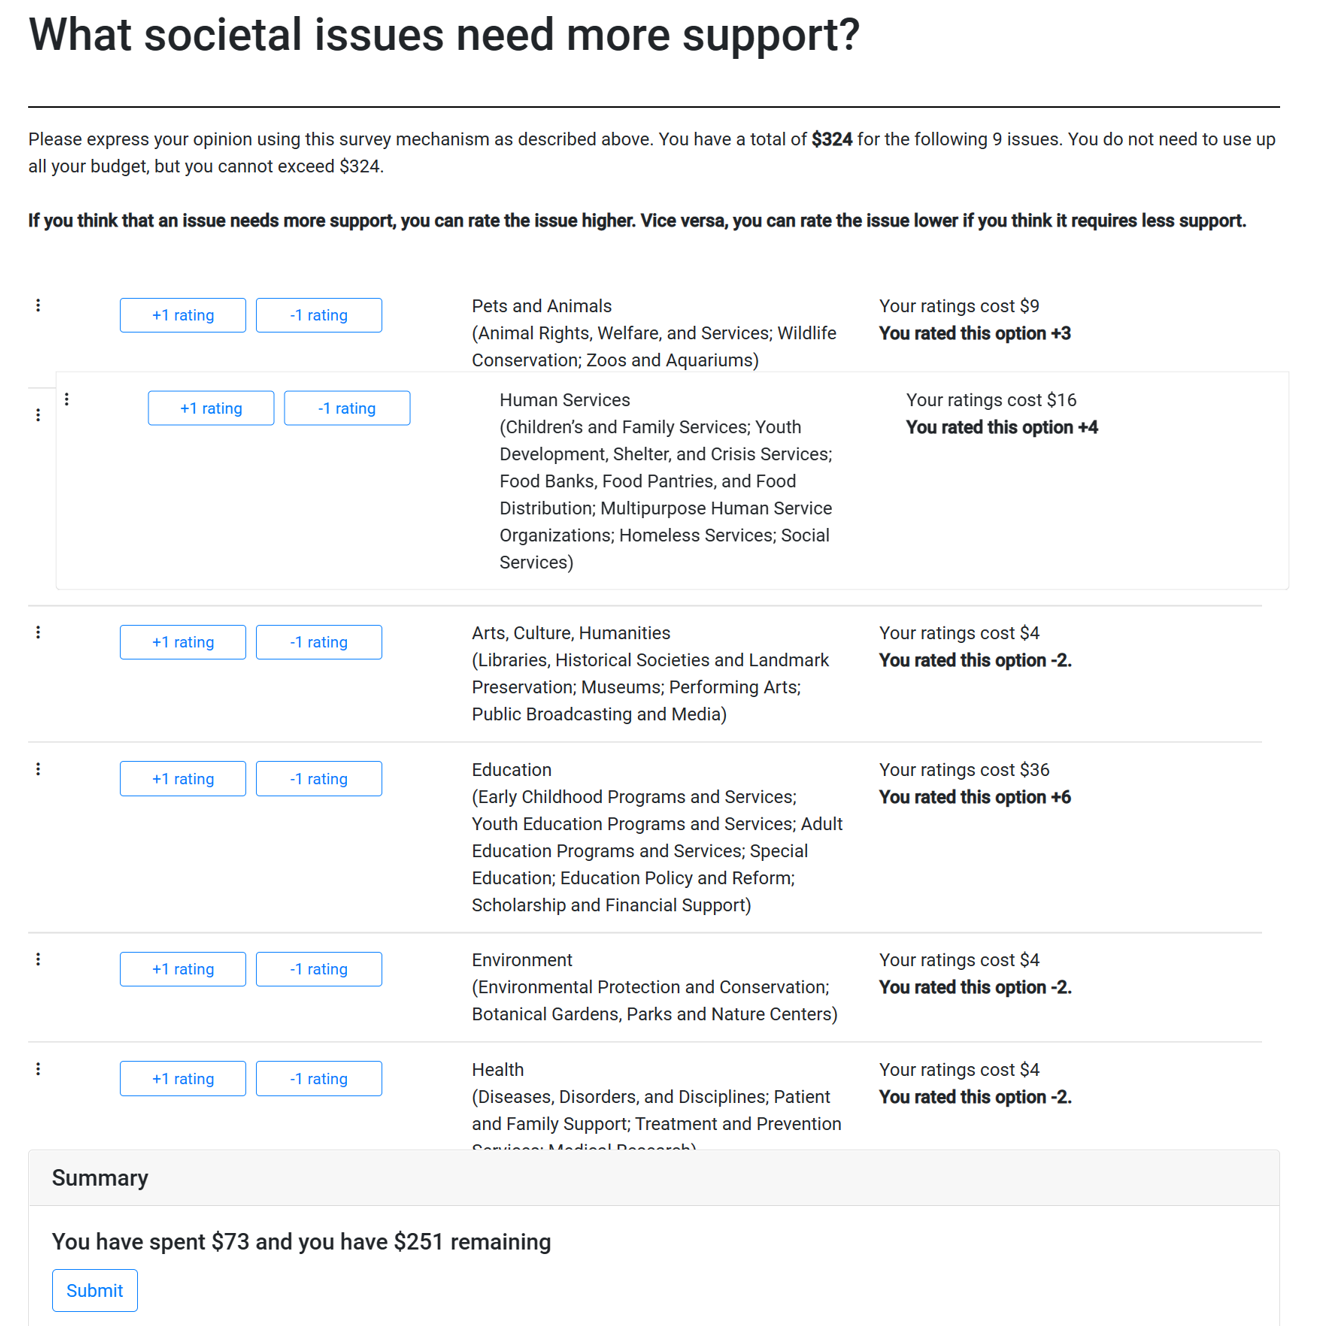
\includegraphics[width=0.43\textwidth]{content/image/prototypes/2_ranking.png}
    \caption{A Ranking-Vote Prototype: The goal of this prototype is to test whether ranking options prior to voting help establish individual's relative preferences, and reduce effort when voting. Each option is draggable to position in a specific location amongst the full list of options. Votes can be updated using the buttons to the right of the interface with vote count and costs to the right of the interface. A summary box is placed sticky to the bottom of the screen.}
    \label{fig:qv_rank}
\end{figure}

\begin{figure}[h]
    \centering
    \begin{subfigure}[b]{0.47\textwidth}
        \centering
        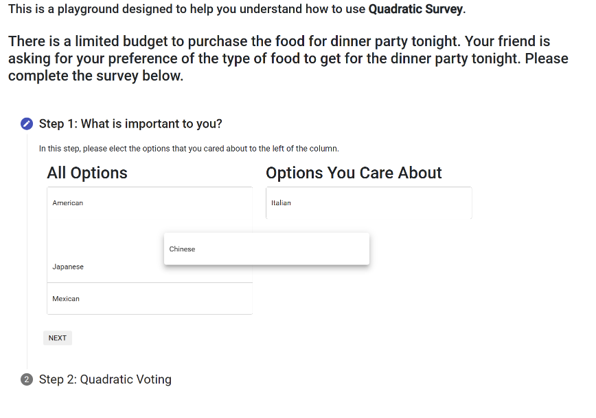
\includegraphics[width=0.9\textwidth]{content/image/prototypes/3.1_selecting.png}
        \caption{Options are dragged and dropped to the 'Option You Care About' box.}
        \label{fig:qv_select_selection}
    \end{subfigure}
    \hfill
    \begin{subfigure}[b]{0.47\textwidth}
        \centering
        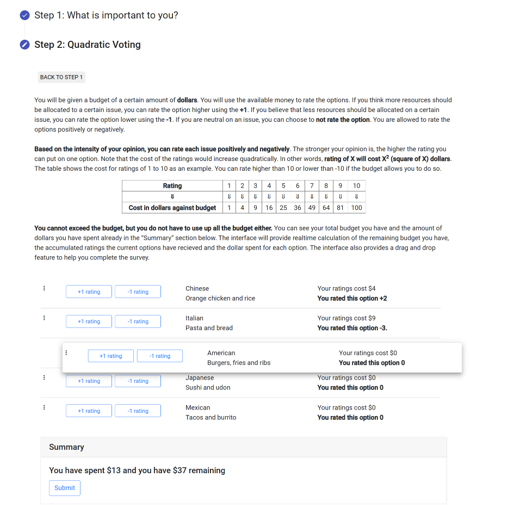
\includegraphics[width=0.9\textwidth]{content/image/prototypes/3.2_selecting_2.png}
        \caption{The previous step collapses showing all voting options.}
        \label{fig:qv_select_vote}
    \end{subfigure}
    \caption{A Select-then-Vote Prototype: The goal of this prototype is to nudge participants to focus on a subset of options to vote, rather than ranking all of them. This prototype introduces a two-step voting process. As shown in Fig.~\ref{fig:qv_select_selection}, the first step involves selecting options for further consideration. Important options are placed at the top of the list for voting shown in Fig.~\ref{fig:qv_select_vote}, but options can be placed anywhere on the list if desired. The rest of the controls remain the same as the previous prototype.}
    \label{fig:qv_select}
\end{figure}

\subsubsection{Prototype 2: Select-then-Vote}
Based on feedback from Prototype 1, instead of \textit{allowing} individuals to rank options, Prototype 2 implemented a two-phase process that \textit{intentionally} asks respondents to select options to express opinions before voting. As shown in Figure~\ref{fig:qv_select}, survey respondents selected their preferred options (Figure~\ref{fig:qv_select_selection}), and the interface positioned these options at the top of the list for voting (Figure~\ref{fig:qv_select_vote}). We identified several issues during prototype 2 pretest: many respondents marked most options as 'options they care about,' which undermined the design's purpose. Additionally, the lack of clear distinction between selected and unselected options confused respondents about the necessity of Step 1. Thus, we need a clearer distinction and connection between the two phases to effectively construct relative preferences.

\begin{figure}[h]
    \centering
    \begin{subfigure}[b]{0.48\textwidth}
        \centering
        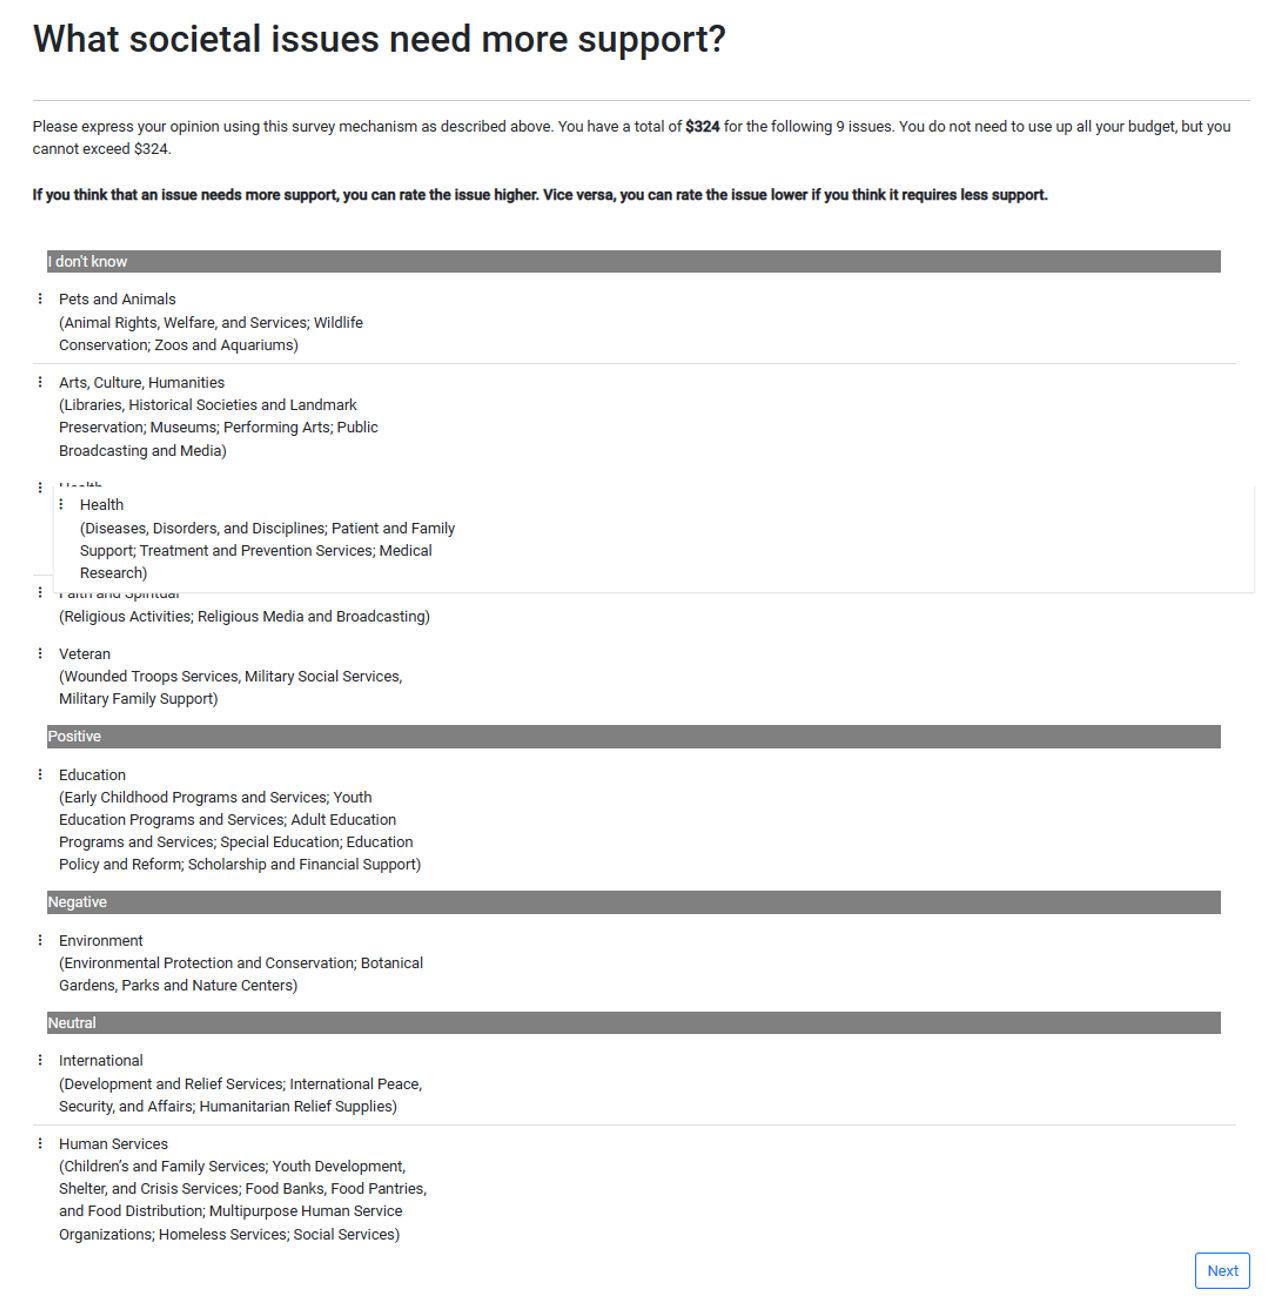
\includegraphics[width=\textwidth]{content/image/prototypes/4.1_grouping.png}
        \caption{The Organization Interface: Options are shown initially in the first bin labeled as `I don't know.' Survey respondents can then drag and drop these options into the latter bins: Positive, Neutral, or Negative. On this interface, only the details of each option are shown.}
        \label{fig:qv_org_p1}
    \end{subfigure}
    \hfill
    \begin{subfigure}[b]{0.48\textwidth}
        \centering
        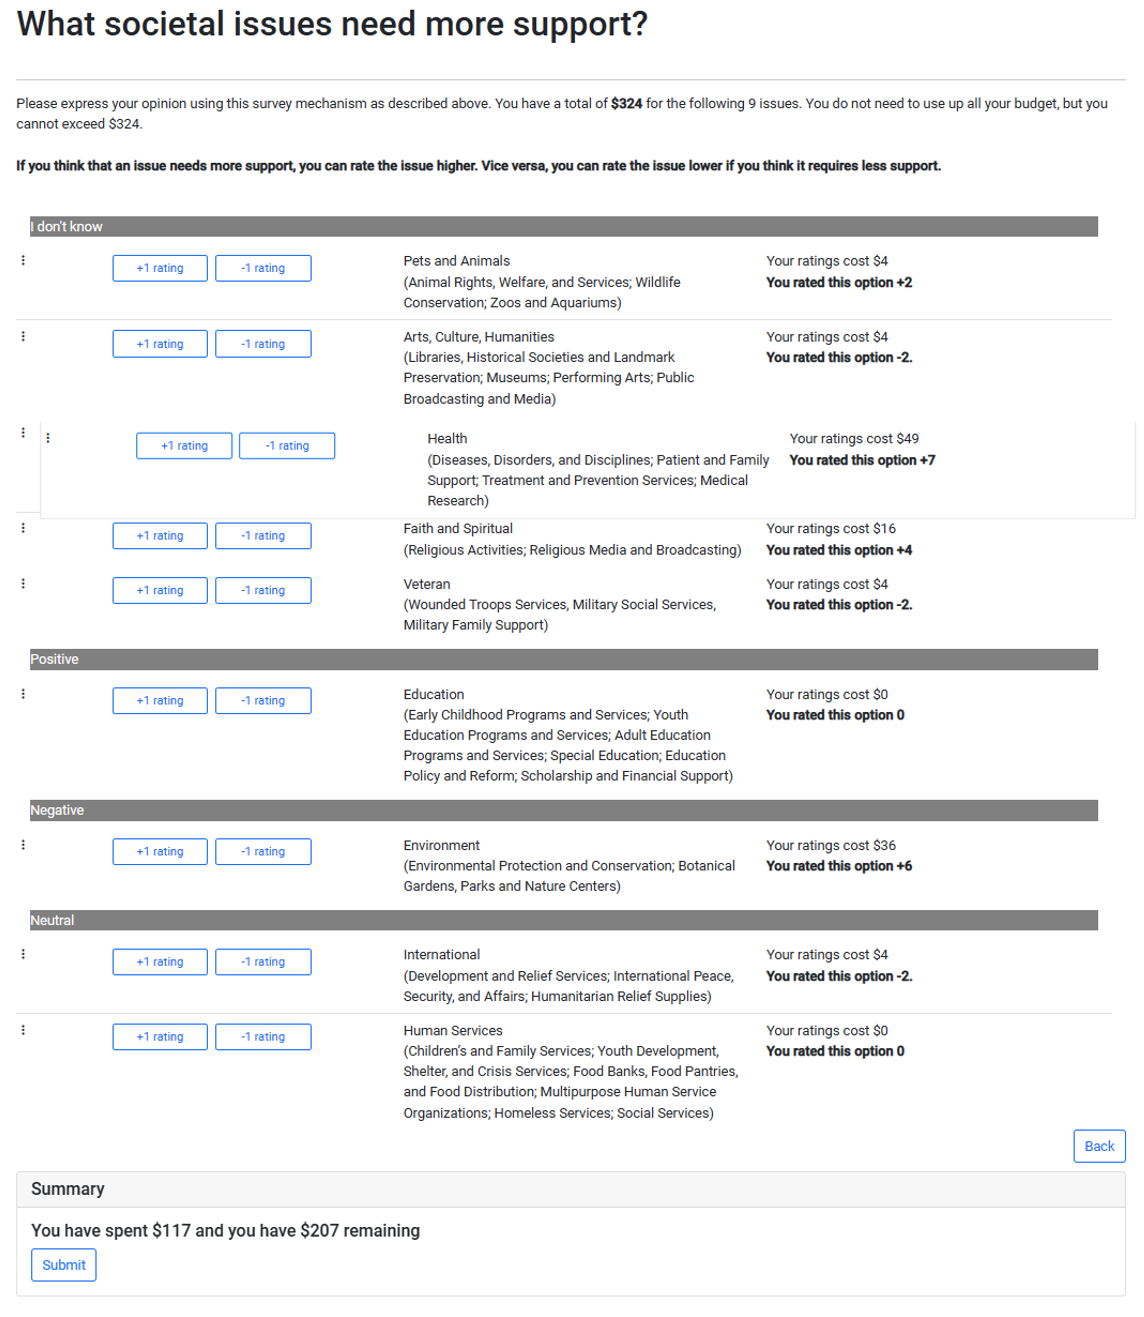
\includegraphics[width=\textwidth]{content/image/prototypes/4.2_grouping_vote.png}
        \caption{The Voting Interface: Voting controls appear on the left side of each option, showing the current votes and associated costs on the right. A budget summary is stuck at the bottom of the screen.}
        \label{fig:qv_org_p2}
    \end{subfigure}
    \caption{Organize-then-Vote Prototype: The goal of this prototype is to encourage participants at deriving finer grain categories among options before voting. Survey respondents first organize their thoughts into categories, then vote on the options.}
    \label{fig:qv_org}
\end{figure}

\subsubsection{Prototype 3: Organize-then-Vote}
Figure~\ref{fig:qv_org} shows the last prototype where we built on the previous takeaway by providing finer-grain groupings and creating a clear connection between option organization and voting position. Specifically, we provided three categories: Positive, Negative, and Neutral. Initially, respondents see all options under the section labeled 'I don't know,' which includes only the option descriptions. We ask respondents to move these options into the categories below. Voting controls and information appear on each option once respondents move to the subsequent page, forming a clear connection between option groups, positions, and voting controls.

Feedback indicated that survey respondents are comfortable with the two-phase organize-then-vote design, demonstrating it as a central strategy for our interface development. However, several areas for enhancement were identified: First, the dragging and dropping mechanism in the organization phase is cumbersome and may inadvertently suggest a ranking process, contrary to our intentions. Second, placing unorganized options at the top of the voting list is counterintuitive. Third, the voting controls are disconnected from the option summaries, dividing attention between the left and right sides of the screen. These insights guided refinements in the final two-phase interface, adhering to the two-phase organize-then-vote design framework.
% ============================= % 

\begin{figure}[ht]
    \centering
    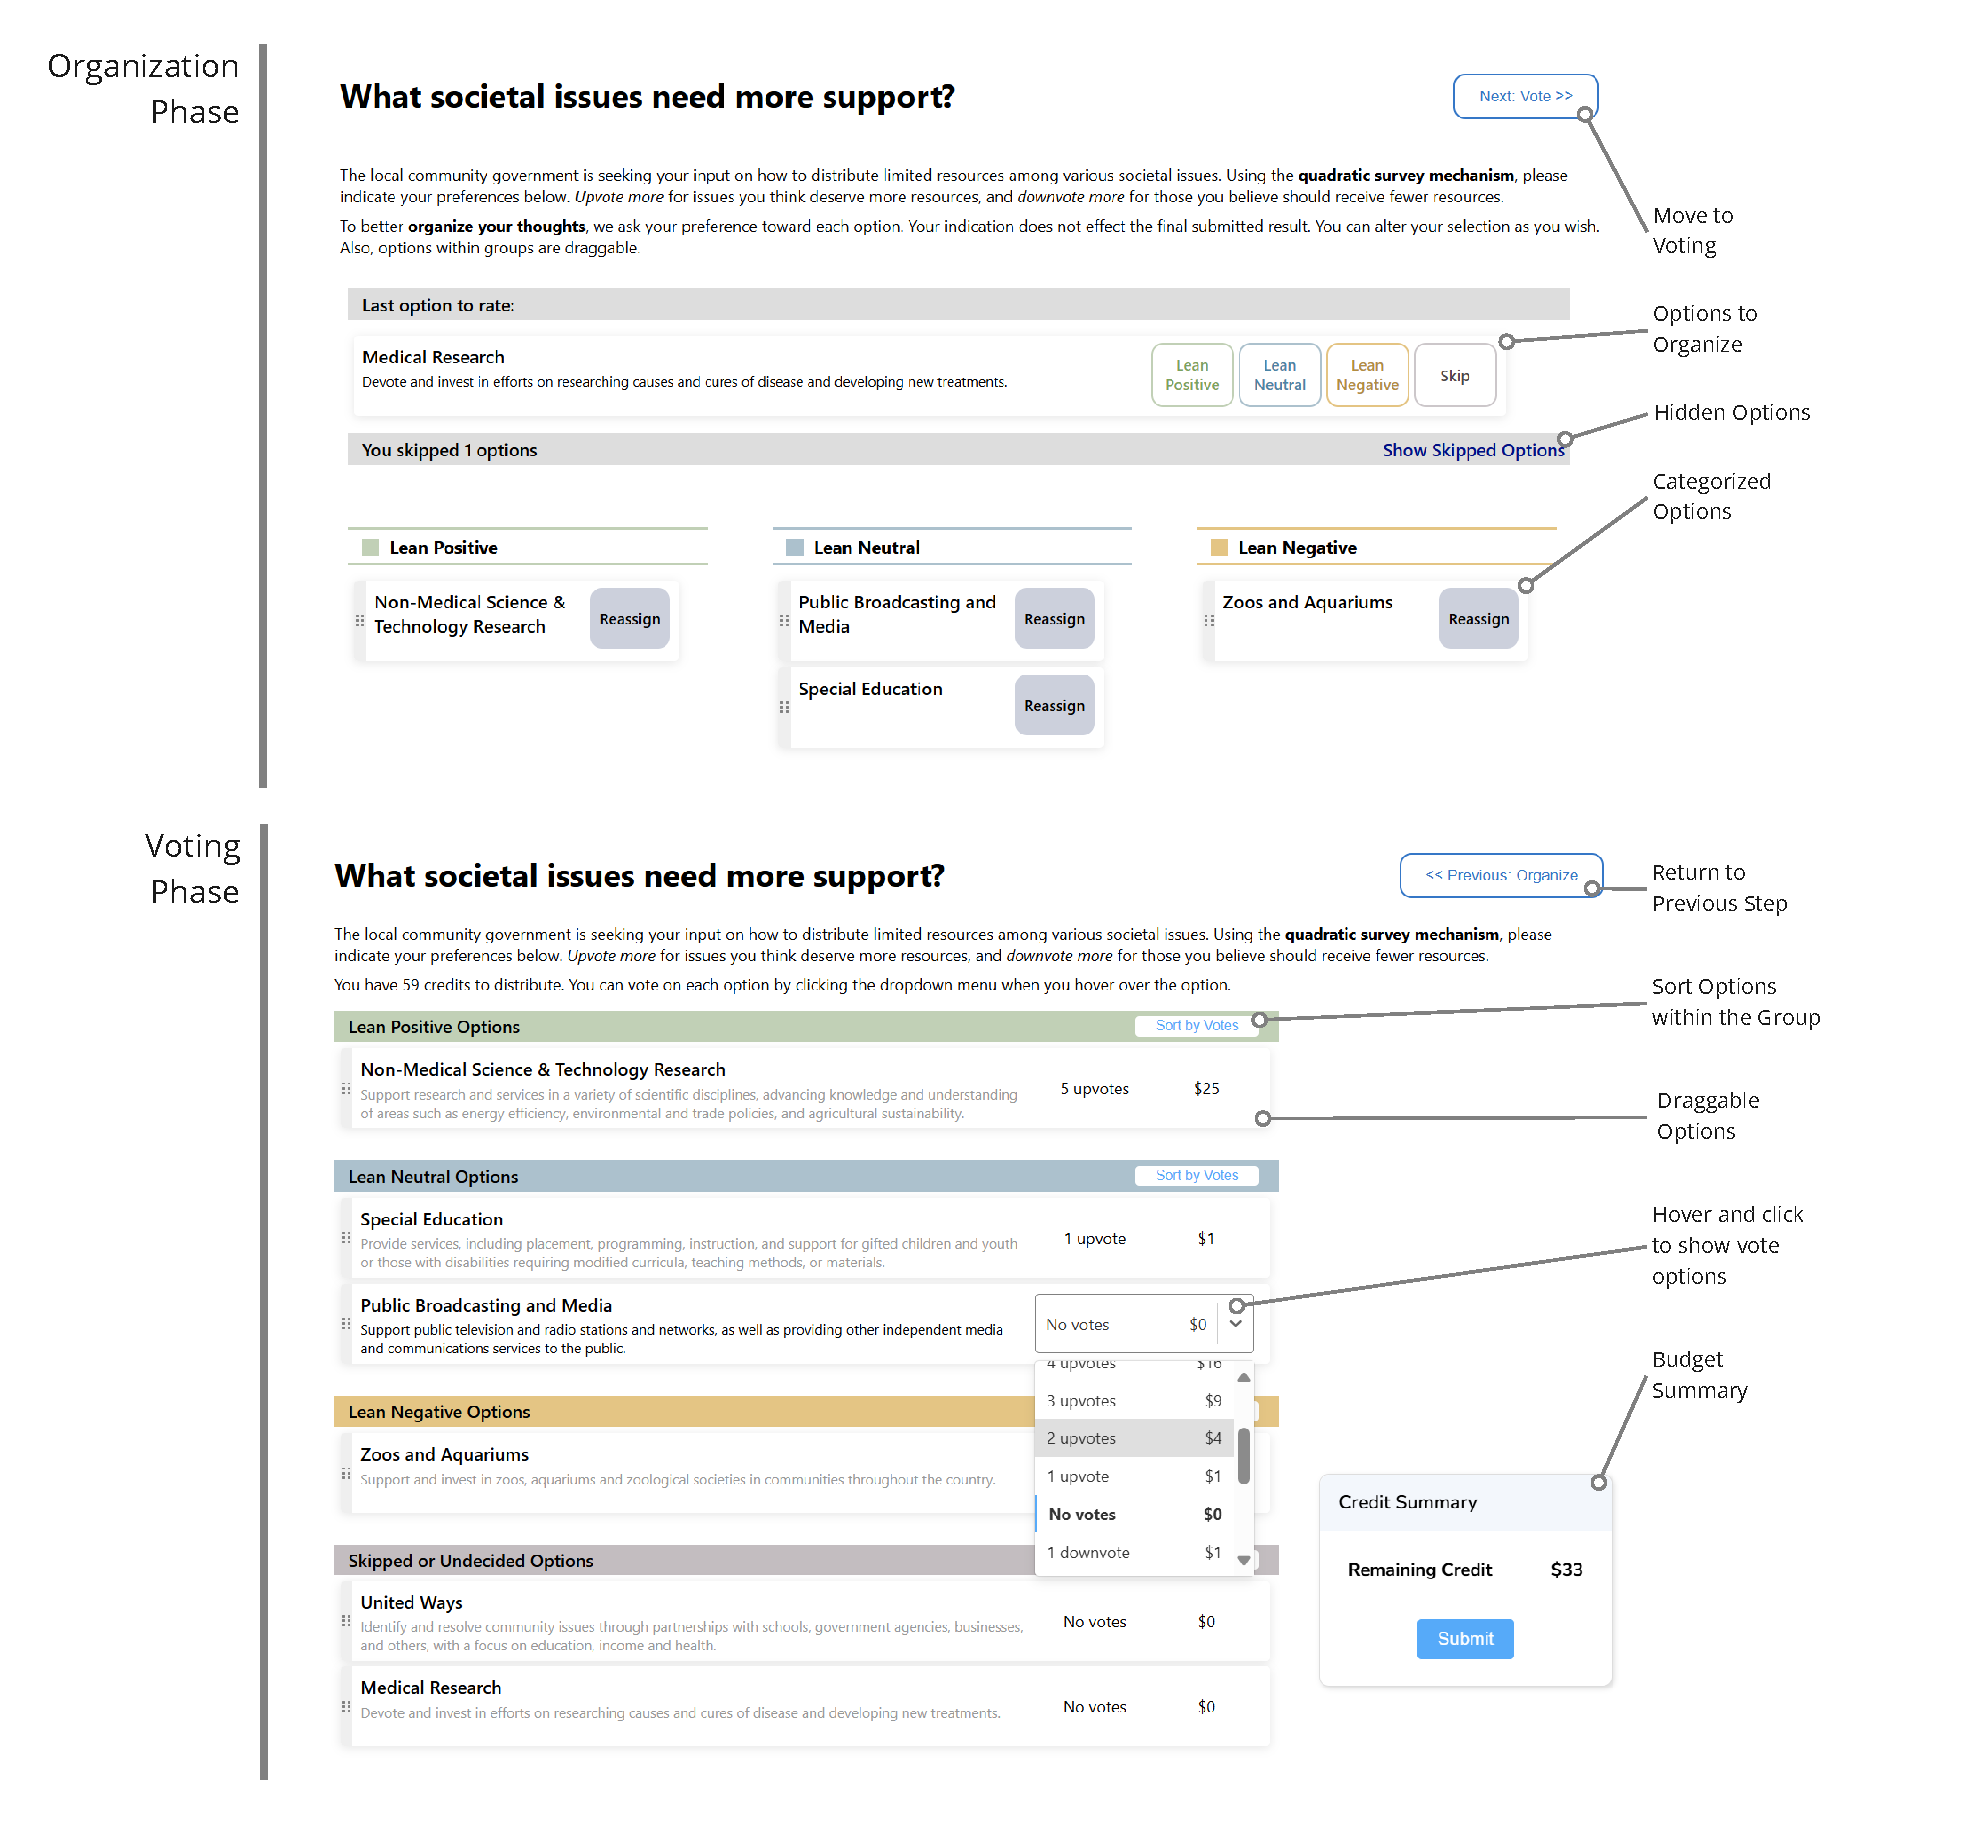
\includegraphics[width=1\textwidth]{content/image/detailed.pdf}
    \caption{The Two-Phase Interface: The interface consists of two phases. Survey respondents can navigate between phases using the top right button. In the organization phase, respondents will be presented with one option at a time where they can choose among four choices: Lean Positive, Lean Neutral, Lean Negative, or Skip. Skipped options are hidden and can be evaluated later. Options that are chosen will be listed below. Items can be dragged and dropped across categories or returned to the stack. In the voting phase, options are listed in the order of the four categories. When hovering over each option, respondents can select a vote for that option using the dropdown. Each dropdown contains the cost associated with the vote. A sort button allows ascending sorting within each category. A summary box tracks the remaining credit balance.}
    \label{fig:interactiveInterface}
\end{figure}

\subsection{Finalizing the Two-Phase Interface}
\label{sec:finalInterfaceDesign}
In the previous subsection, we highlighted critical prototype iterations that informed the final two-phase interactive process that defines the user journey. 
We now present the final two-phase interface, its operations, and the supporting literature for comprehensive understanding.
Then, We also discuss the aesthetic design choices that emerged throughout the iterations.

\subsubsection{Justifying a two-phase approach}
Recall the ultimate objective of the two-phase interface is to facilitate preference construction and reduce cognitive load. The two-phase interface, shown in Figure~\ref{fig:interactiveInterface} consists of two steps: An organization phase and a voting phase. Throughout both phases, survey respondents can drag-and-drop options across the presented option list.

\paragraph{A two-phase approach}
If preferences are constructed, by nature, they consist of a series of constructed decision-making processes~\cite{lichtensteinConstructionPreference2006}. Two major decision-making theories informed the design decision of a two-step interaction interface design:~\textcite{montgomeryDecisionRulesSearch1983}'s Search for a Dominance Structure Theory (Dominance Theory) and~\textcite{svensonDifferentiationConsolidationTheory1992}'s Differentiation and Consolidation Theory (Diff-Con Theory). The former suggested that decision-makers prioritize creating dominant choices to minimize cognitive effort by focusing on evidently superior options~\cite{montgomeryDecisionRulesSearch1983}. The latter described a two-phase process where decisions are formed by initially ~\textit{differentiating} among alternatives and then~\textit{consolidating} these distinctions to form a stable preference~\cite{svensonDifferentiationConsolidationTheory1992}. Both theories echoed the design decision in building the interactive experience to reduce initial decision dimensions and the mental procedures involved in emphasizing relatively important options and forming decisions.

Hence, the two-phase design -- organize then vote -- aimed to facilitate this cognitive journey explicitly. The first phase focused on differentiating and identifying dominant options, enabling survey respondents to preliminarily categorize and prioritize their choices. The second phase presented these categorized options in a comparable manner, with drag-and-drop functionality, enhancing one's ability to consolidate preferences. This structured approach aimed to construct a clear decision-making procedure that reduced cognitive load and enhanced clarity and confidence in the decisions made.

\paragraph{Phase 1: Organization Phase}
The goal of the organization phase was to support participants in identifying dominating options or partitioning options into differentiable groups. In this section, we first describe how the interaction worked, then we detail reasons for the different design decisions implemented.

The organizing interface, depicted on the top half of Figure~\ref{fig:interactiveInterface}, sequentially presented each survey option. Participants selected a response among three ordinal categories -- lean positive, lean negative, or lean neutral. Once selected, the system moved that option to the respective category. Participants could skip the option if they did not want to indicate a preference. Options within the groups were draggable and rearrangeable to other groups should the participants wish.

\textcite{strackThinkingJudgingCommunicating1987}'s research showed that upon understanding a survey question, respondents either recalled a prior judgment or constructed a new one when completing an attitude survey. In addition, revealing one option at a time gated the amount of information presented to the survey respondent and thereby reduced the extraneous load~\cite{swellerCognitiveLoadTheory2011}. This process allowed participants to form or express opinions on individual options incrementally. This design also mitigated the original concern from prototype 3 where participants accidentally treated the organizing task as a ranking task.

The three possible options, positive, neutral, and negative, aimed to scaffold participants in constructing their own choice architecture~\cite{munscherReviewTaxonomyChoice2016, thalerNudgeImprovingDecisions2008a}, which strategically segmented options into diverse and alternative choice presentations while avoiding the biases from defaults. We believed that these three categories were sufficient for participants to segment the options. However, we chose not to limit the number of options one could place into a category to prevent restricting user agency, a core user interface design principle~\cite{norman2013design}.

Immediate feedback displaying the placement of options and allowing participants to rearrange them via drag-and-drop adhered to key interface design principles~\cite{norman2013design}. At the same time, it allowed finer grain control for individuals to surface dominating options and create differentiating groups of options.

\paragraph{Phase 2: Interactive Voting Phase}

The objective of the voting phase was to facilitate the consolidation of differentiated options through interactive elements while reinforcing the differentiation across options constructed by participants from the previous phase. This facilitation was achieved by retaining the drag-and-drop functionality for direct manipulation of position and enabling sorting within each category.

Options were displayed as they were categorized within each category from the previous step and in the following section orders -- lean positive, lean neutral, lean negative, and skipped or undecided as detailed on the bottom half of Figure~\ref{fig:interactiveInterface}. The Skipped or Undecided category contained options left in the organization queue, possibly because survey respondents had a pre-existing preference or chose not to organize their thoughts further. The original order within these categories was preserved to maintain and reinforce the differentiated options. This new ordering sequence mitigated the concern from prototype 3 where options without a category are left at the top of the voting interface. Respondents had the flexibility to return to the organization interface at any point during the survey to revise their choices.

In the voting interface, options remained draggable, enabling participants to modify or reinforce their preference decisions as needed. Each category featured a sort-by-vote function that enabled reordering within the same category. Although these interactions did not influence the final voting outcome, they were designed to support consolidation and positional proximity in information organization. This design aimed to automate the grouping of similar options while providing an intuitive drag-and-drop mechanism, thereby facilitating decision-making by placing similar options near each other. This echoed the principles of the proximity compatibility principle, particularly emphasizing spatial proximity and mental compatibility~\cite{wickens1990proximity}. The interface design anticipated that participants would find it easier to consolidate their choices when similar options were positioned close together, thereby reducing cognitive load.

While multiple interaction mechanisms exist, drag-and-drop has been extensively explored in rank-based surveys. For instance,~\textcite{krosnick2018measurement} demonstrated that replacing drag-and-drop with traditional number-filling rank-based questions improved participants' satisfaction with little trade-off in their time. Similarly,~\textcite{timbrook2013comparison} found that integrating drag-and-drop into the ranking process, despite potentially reducing outcome stability, was justified by the increased satisfaction and ease of use reported by respondents. The trade-off was deemed worthwhile as QS did not use the final position of options as part of the outcome if it significantly enhanced user satisfaction and usability~\cite{rintoulVisualAnimatedResponse}.

Together, these design decisions led to our belief that a two-phase interface with direct interface manipulation could reduce the cognitive load for survey respondents to form preference decisions when completing QS.

\subsubsection{Aesthetic Design Decisions}
There are three aesthetic design decisions that made it to the final interface. First, we decided to remove all visual elements. Prior literature suggested that the use of emojis might influence the interpretations of surveys~\cite{herringGenderAgeInfluences2020} and decrease user satisfaction~\cite{toepoelSmileysStarsHearts2019}. Prior literature also noted that not all data visualization elements reduce cognitive demand~\cite{huangMeasuringEffectivenessGraph2009a}. Even though effective visualization can aid decision-making, it remains an open question that this study does not aim to address, thus we also removed all visualization elements such as blocks, progress bars, and percentage indicators.

Second, the final interface has all options presented on the screen at the same time, intentionally. Unlike all the prototypes and existing interfaces, prior literature emphasized the importance of placing all the options on the same digital ballot screen to avoid losing votes. This echoes the proverb "out of sight, out of mind," where individuals might be biased toward options that are shown to them, and additional effort is required for individuals to retrieve specific information if options are hidden.

Last, we decided to use a dropdown positioned to the right of the option such that control of votes and the budget summary are placed near one another. The layout of the votes and cost was inspired by online shopping cart checkout interfaces where quantities are supplied next to the itemized costs followed by the total checkout amount. We chose a dropdown after iterating with two alternative input methods (Figure~\ref{fig:btn_design}): the original click-based buttons and a wheel-based implementation. The former design requires survey respondents to click multiple times to reach their desired vote values. Thus, we wanted to look for a solution to aid respondents in reaching their intended value faster. A wheel-based approach allows intuitive control of the votes by using the wheel on the mouse and clicking to fine-tune the values. However, in our early pilot studies, not all participants were familiar with wheel control, thus we opted for a dropdown menu for vote selection.

\begin{figure}[h]
    \centering
    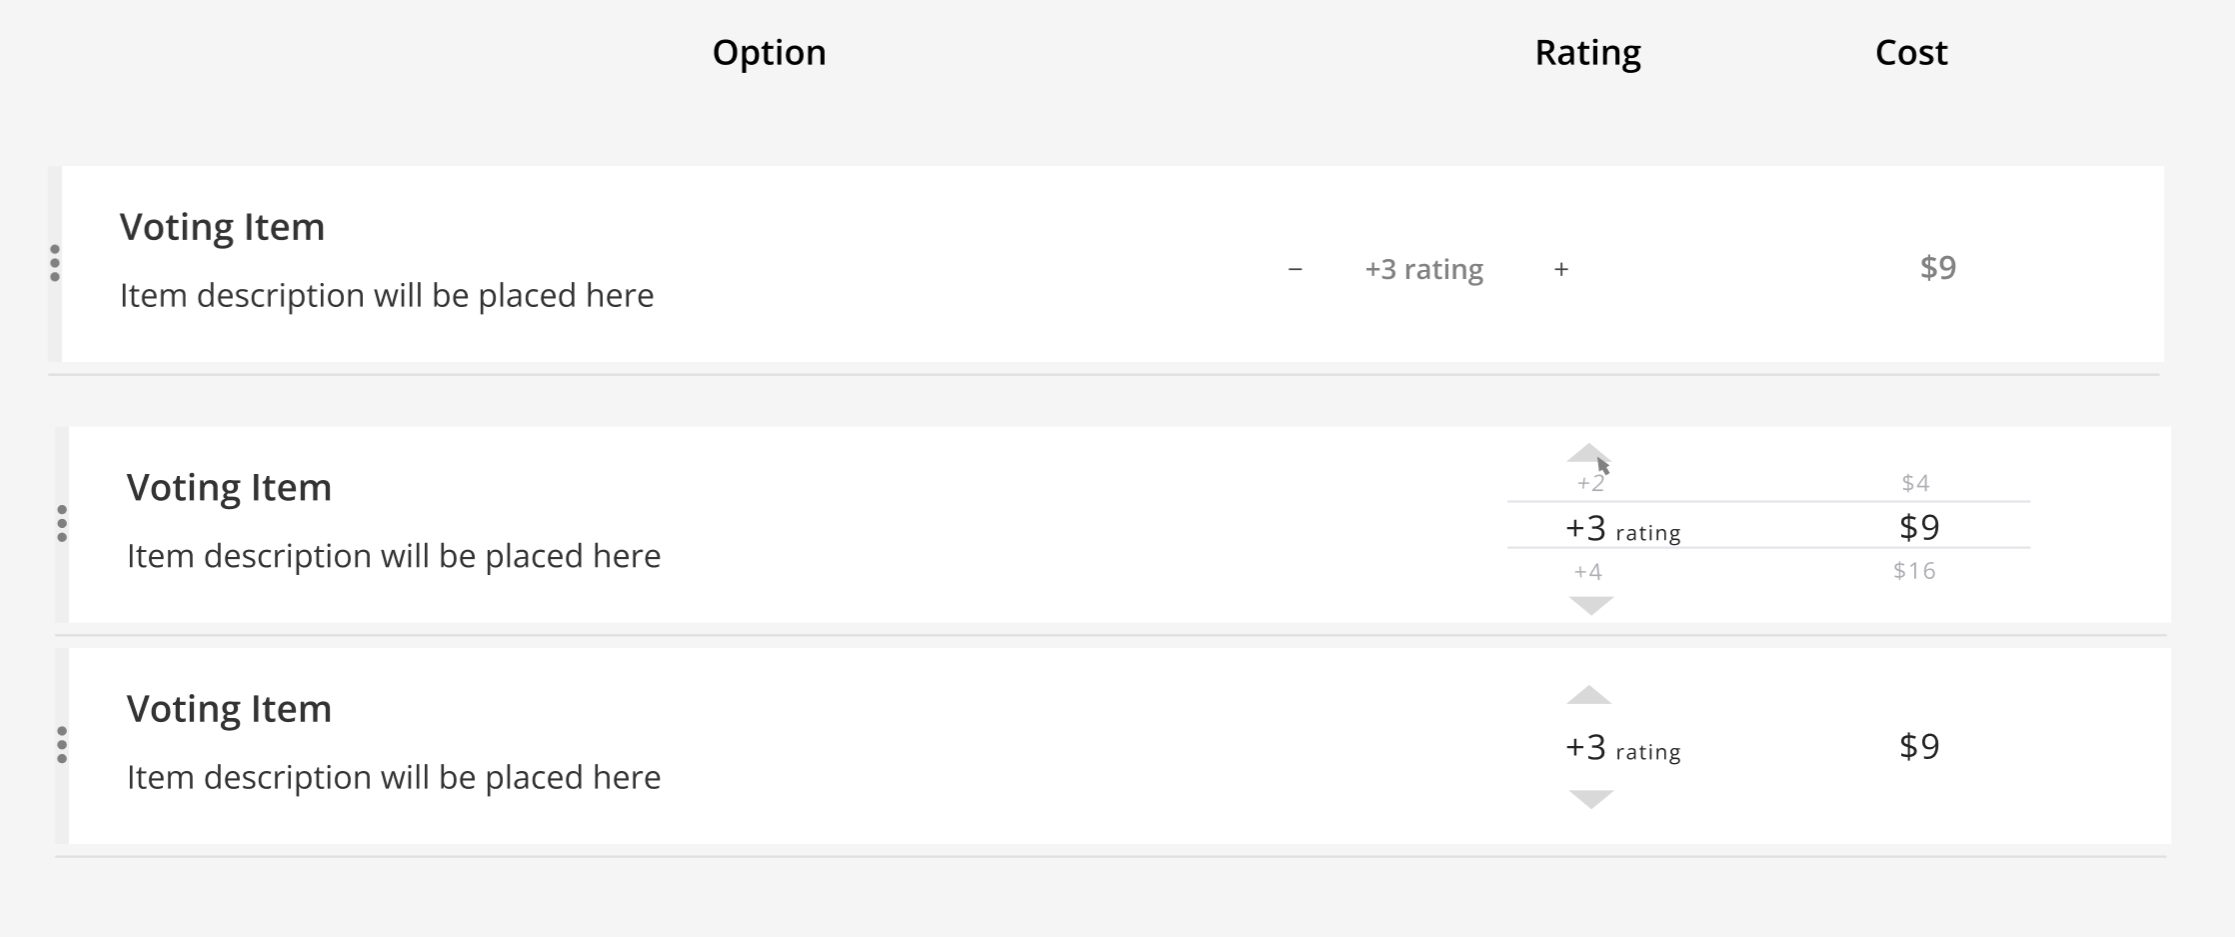
\includegraphics[width=0.8\textwidth]{content/image/prototypes/btn_design.png}
    \caption{The click-based and wheel-based designs for vote control included: The former mirrors traditional vote control used in other quadratic voting interfaces, where each click represents an increase in votes. The latter allows control through both clicks and mouse wheel rotation.}
    \label{fig:btn_design}
\end{figure}

\begin{figure}[h]
    \centering
    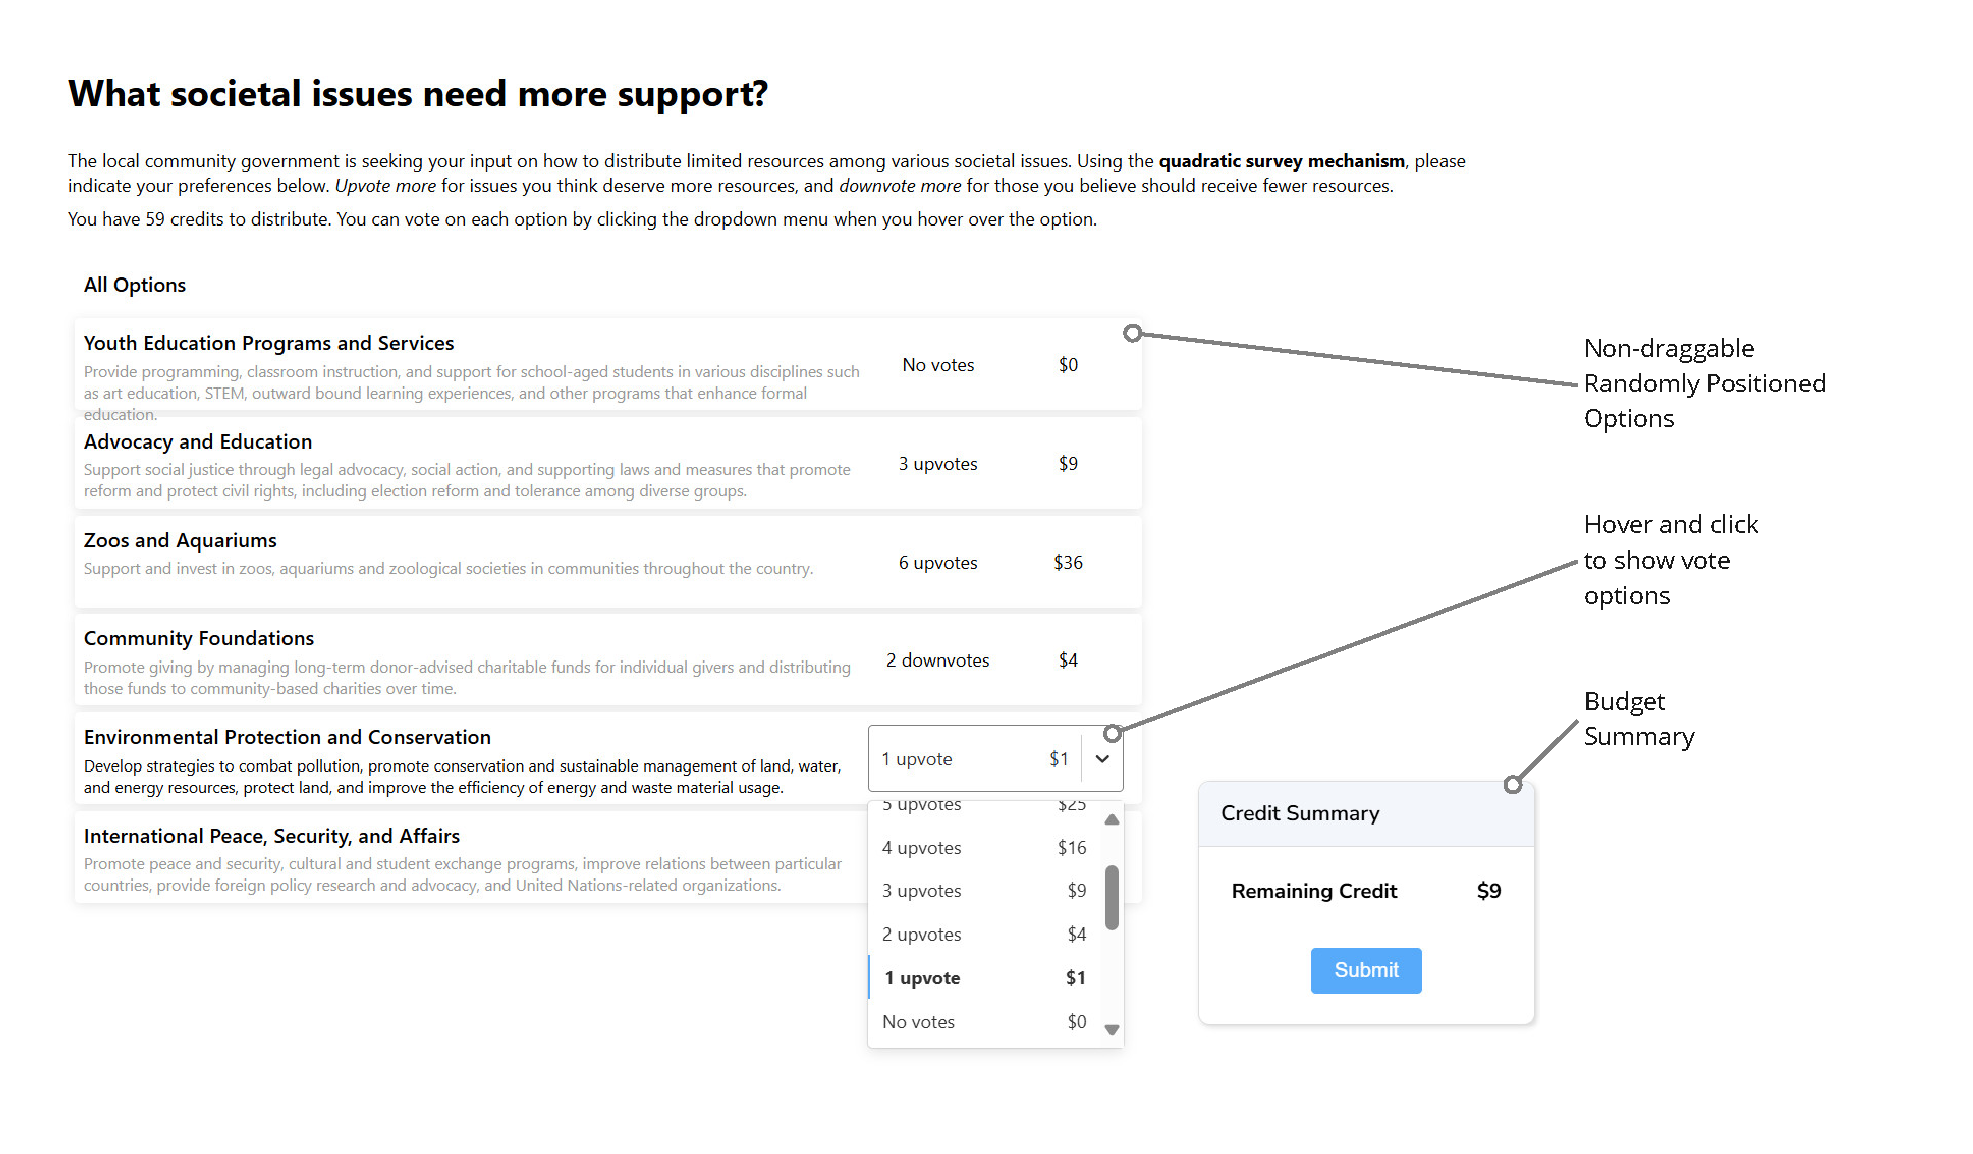
\includegraphics[width=\textwidth]{content/image/detailed_text.pdf}
    \caption{The text-based interface: This interface is based on the interactive version but does not include the two-phase interactive support and lacks the drag-and-drop functionality. Options are randomly positioned.}
    \label{fig:textInterface}
\end{figure}

\subsection{Text-based Interface} To study how the interactive components influenced participants' cognitive load and behavior, we removed the two-phase interactive design and the drag-and-drop features for the text-based interface. The text-based interface shares the other functionalities of the two-phase interface, as shown in Figure~\ref{fig:textInterface}. The interface contained the question prompt at the top of the screen. The options were presented in a list underneath the prompt. Survey respondents could update the votes by selecting from a dropdown that provided all possible voting options and costs given the number of credits available. A small summary box to the right of the interface showed the current total cost and the remaining credits for the respondent. The interface randomly presented options to avoid ordering bias~\cite{ferberOrderBiasMail1952, couperWebSurveyDesign2001}.

Both experiment interfaces are developed with a React.js frontend and a Next.js backend powered on MongoDB. Both services were open-sourced~\footnote{link-to-github}.



% In our first prototyped tool, we aim to help survey respondents rank options to establish relative preferences before voting. As shown in Figure~\ref{fig:qv_rank}, our prototype allows respondents to move options before finalizing their votes. During our pretest, we found that respondents rarely moved the options and some questioned the need for a full ranking since it did not affect the QS submission. Many did not realize the options were draggable until we pointed it out. The main insight from this prototype is that creating a full rank is~\textit{not} essential for establishing~\textit{relative} preferences, leading us to consider selecting a subset of options instead of requiring a full rank among all options.

% First, we surveyed the current implementation of QV interfaces to understand the development of such tools. We presented a selection in Figure~\ref{fig:qv_interface_external}. All five interfaces retained and presented the following components:
% \begin{itemize}
%     \item Option list: A list of options contesting for votes.
%     \item Vote Controls: Two buttons to increase and decrease votes associated with each option.
%     \item Individual vote tally: A representation of votes associated with an option.
%     \item Summary: A summary that automatically calculated the cost across options and the remaining budget.
% \end{itemize}
% Now we present the final interactive interface and describe how it operates. In this subsection, we provide supporting evidence from prior literature that we previously omitted. These pieces of literature were omitted for clarity and focus in the previous subsection but will be reintroduced here. 
% We constructed a text-based interface that included all five components but removed the use of emojis (i.e., thumbs up and thumbs down present in Figure~\ref{fig:wedesignInterface}), progress bars, and other visualizations in the summary section (i.e., progress bars in Figure~\ref{fig:wedesignInterface} and~\ref{fig:chengInterface} or blocks presented in Figure~\ref{fig:rxcvotingInterface}), and the visual cues for individual vote counts (i.e., the colored counts and icons present in Figure~\ref{fig:gov4gitInterface} and~\ref{fig:chengInterface}).

% During this process, we noticed several issues. First, many survey respondents placed most options into the 'option you care about' category, defeating the design's purpose. Second, there were no indicators distinguishing between the selected and remaining options. Respondents did not notice their selections were kept at the top in the voting stage and were unsure why Step 1 was necessary if all options were shown again. This informed two takeaways: selecting options to vote on is too coarse to construct relative preferences, and there needs to be a clearer distinction and connection between the two phases.

% Feedback indicated that survey respondents are comfortable with this two-phase organize-then-vote design. Several user experience issues emerged, but they were addressable without significantly modifying this interaction structure. These issues include: First, dragging and dropping all options into different categories is cumbersome and can mislead respondents into thinking this is a ranking process, which is not the goal. Second, the position of unorganized options at the top of the voting list is counterintuitive. Third, the voting controls are disconnected from the option summaries, dividing attention between the left and right sides of the screen.

% These design decisions led to the interface shown in Figure~\ref{fig:textInterface}. 


% \subsubsection{Paper prototype: visualizing trade-offs}
% The original paper prototype aimed to help visualize survey respondents' tradeoffs among options. 
% The original paper prototype aimed to utilize visual representations to highlight the constrained availability of credit and to explain the costs and trade-offs associated with selecting each available option.
% Early on, we did not know which components made QS more difficult than other survey techniques. We began by surveying existing interfaces (Figure~\ref{fig:qv_interface_external} other than Figure~\ref{fig:gov4gitInterface} which did not exist near the writing of this paper). All four interfaces consist of these common components:
% As we were unsure what made QS more complex than other survey techniques, our investigation began with the existing interface (Figure~\ref{fig:qv_interface_external}, except Figure~\ref{fig:gov4gitInterface} which did not exist at that time. All four interfaces consist of these common components:
% \begin{itemize}
%     \item Option list: A list of options contesting for votes.
%     \item Vote Controls: Buttons to increase and decrease votes associated with each option.
%     \item Individual vote tally: A representation of votes associated with an option.
%     % \item Summary: A summary that automatically calculates the cost across options and the remaining budget.
%     \item Summary: An auto-generated summary of costs and remaining budget.
% \end{itemize}

% To brainstorm ways to help survey respondents manage trade-offs across options, we decomposed these options and explored several innovative layouts. Initially, we thought trade-offs were the core cause of cognitive load. In this paper, we show two versions of the paper prototypes in Figure~\ref{fig:qv_paper}. In both figures, costs are represented by blocks, similar to Figure~\ref{fig:rxcvotingInterface}. We imagine the survey respondents to drag and position options in the space provided unstructurally (Figure~\ref{fig:horizontal_paper}) or structurally (Fig~\ref{fig:vertical_paper}). Similar to the seminal debate on direct manipulation vs. interface agents~\cite{shneidermanDirectManipulationVs1997}, the research team was unsure how much control survey respondents should have over the positioning of the options to aid the decision-making process that considers trade-offs. Different from prior interfaces, we used placements of the interface to denote positive or negative number of votes. After several pretests, we learned that the main process participants aim to do throughout the survey is establishing~\textit{relative} preferences across the options, rather than thinking so much about trade-offs. 
% To further explore the features that contribute most to the complexity of QS, we developed two prototypes shown in Figure~\ref{fig:qv_paper}. Similar to Figure~\ref{fig:rxcvotingInterface}, these prototypes use blocks to represent costs, arranged either unstructurally (Figure~\ref{fig:horizontal_paper}) or structurally (Fig~\ref{fig:vertical_paper}), facilitating the visualization of the trade-offs. Unlike previous interfaces, we utilized the placement of the interface to denote positive or negative vote counts. Several protests indicated that participants primarily focus on establishing relative preferences among options rather than trade-offs. Therefore, in this study, we focused on enhancing designs that facilitate the establishment of relative preferences.
% the two main features of QS we identified are the relative preference through a combined presentation of rankings and ratings, and the option selection trade-offs due to total credit limits. 
% The initial prototyping involves collecting the interface designs for existing quadratic mechanism-based software. Iterative pretests informed each subsequent design. We present these iterations, which aim to enhance user experience in the preference construction process in the following sections.